\documentclass[a4paper, 14pt]{extarticle}
\usepackage[margin=1in]{geometry}
\usepackage{amsfonts, amsmath, amssymb}
\usepackage[none]{hyphenat}
\usepackage{fancyhdr} %create a custom header and footer
\usepackage[utf8]{inputenc}
\usepackage[english, main=ukrainian]{babel}
\usepackage{pgfplots}
\usepgfplotslibrary{fillbetween,colormaps}
\usepackage{bm}
\usepackage{physics}
\usepackage[unicode]{hyperref}
\usepackage{scalerel,stackengine}
\usepackage{tikz-cd}
\usetikzlibrary{calc,patterns,angles,quotes, matrix}

\usepackage{tikz-3dplot}
\usetikzlibrary{fit,matrix}

\fancyhead{}
\fancyfoot{}
\parindent 0ex
\def\huge{\displaystyle}
\def\defin#1{\textbf{Definition {#1}}}
\def\ex#1{\textbf{Example {#1}}}
\def\rm#1{\textbf{Remark {#1}}}
\def\prp#1{\textbf{Proposition {#1}}}
\def\lm#1{\textbf{Lemma {#1}}}
\def\th#1{\textbf{Theorem {#1}}}
\def\crl#1{\textbf{Corollary {#1}}}
\def\proof{\textbf{Proof.}\\}
\def\proofMI{\textbf{Proof MI.}\\}
\def\bigline{\vspace{5mm}\\}
\def\qed{$\blacksquare$}
\def\dim#1{\textrm{dim} {#1}}
\def\ker#1{\textrm{Ker} {#1}}
\def\contra{\textbf{!}}




\begin{document}
	\begin{titlepage}
		\begin{center}
		\hfill
		\vfill
		\line(1,0){400}\\
		\large{\textbf{Аналітична геометрія}}\\[1mm]
		{\textbf{Семестр 1}}\\[1mm]
		\line(1,0){400}\\
		\vfill
        	\end{center}
    	\end{titlepage}
\tableofcontents
\newpage
	
	\section{Вектори}
	\subsection{Основні означення}
	\defin{1.1.1. Вектор} - напрямлений відрізок\\
	Позначення: $\vec{a}$
	\hspace{1cm}
	\begin{tikzpicture}
	\draw[thick, ->] (0,0)--(2,1) node at (1,1) {$\vec{a}$};
	\end{tikzpicture}
	\bigline
	\defin{1.1.2.} Два вектора, що лежать на паралельних прямих (або на одній прямій), називають \textbf{колінеарними}\\
	Позначення: $\vec{a} \parallel \vec{b}$\\
	\\
	Інші позначення для колінеарних векторів: \\ 
	$\vec{a} \uparrow \uparrow \vec{b}$ - співнапрямлені вектори\\
	$\vec{a} \uparrow \downarrow \vec{b}$ - протилежно напрямлені вектори\\
	\\
	$|\vec{a}|$ - довжина вектора
	\\
	\\
	\defin{1.1.3.} Вектори $\vec{a}$ та $\vec{b}$ називають \textbf{рівними}, якщо:
	\begin{align*}
	\textrm{-  } \vec{a} \uparrow \uparrow \vec{b} \\
	\textrm{-  } |\vec{a}| = |\vec{b}|
	\end{align*}
	\defin{1.1.4.} Задані операції над векторами:\\
	- \textbf{додавання};\\
	\begin{tikzpicture}
	\draw[thick, ->] (0,0)--(2,2) node at (1,1.5) {$\vec{a}$};
	\draw[thick, ->] (2,2)--(4,2) node at (2.5,2.5) {$\vec{b}$};
	\draw[thick, red, ->] (0,0)--(4,2) node at (2,0.5) {$\vec{a}+\vec{b}$};
	\node at (2,-1) {правило трикутника};
	\end{tikzpicture}
	%
	\hspace{1cm}
	\begin{tikzpicture}
	\draw[thick, ->] (0,0)--(2,2) node at (1,1.5) {$\vec{a}$};
	\draw[thick, ->] (0,0)--(2,0) node at (1,-0.5) {$\vec{b}$};
	
	\draw[thick, dashed] (2,2)--(4,2);
	\draw[thick, dashed] (2,0)--(4,2);
	\draw[thick, red, ->] (0,0)--(4,2) node at (3,1) {$\vec{a}+\vec{b}$};
	\node at (2,-1) {правило паралелограма};
	\end{tikzpicture}
	\bigline
	- \textbf{множення на скаляр;}\\
	\begin{tikzpicture}
	\draw[thick, red, ->] (0,0)--(4,2) node at (3,1) {$\lambda \vec{a}$};
	\draw[thick, ->] (0,0)--(2,1) node at (1,1) {$\vec{a}$};
	\draw[white] (0,-1)--(2,-1);
	\node at (2,-2) {$\lambda > 0$};
	\end{tikzpicture}
	%
	\hspace{1cm}
	\begin{tikzpicture}
	\draw[thick, red, ->] (0,0)--(-4,-2) node at (-3,-1) {$\lambda \vec{a}$};
	\draw[thick, ->] (0,0)--(2,1) node at (1,1) {$\vec{a}$};
	\draw[white] (0,-1)--(2,-1);
	\node at (-1,-2) {$\lambda < 0$};
	\end{tikzpicture}
	\bigline
	А також задані наступні властивості:\\
	$\forall \vec{a}, \vec{b}, \vec{c}: \forall \lambda, \mu \in \mathbb{R}:$\\
	1) $\vec{a} + \vec{b} = \vec{b} + \vec{a}$\\
	\begin{tikzpicture}
	\draw[thick, ->] (0,0)--(2,2) node at (1,1.5) {$\vec{a}$};
	\draw[thick, ->] (2,2)--(4,2) node at (2.5,2.5) {$\vec{b}$};
	\draw[thick, red, ->] (0,0)--(4,2) node at (2,0.5) {$\vec{a}+\vec{b}$};
	\end{tikzpicture}
	%
	\hspace{1cm}
	\begin{tikzpicture}
	\draw[thick, ->] (2,0)--(4,2) node at (2.5,0) {$\vec{a}$};
	\draw[thick, ->] (0,0)--(2,0) node at (1.5,0.5) {$\vec{b}$};
	\draw[thick, red, ->] (0,0)--(4,2) node at (2,1.6) {$\vec{b}+\vec{a}$};
	\end{tikzpicture}
	\\
	\\
	2) $(\vec{a} + \vec{b}) + \vec{c} = \vec{a} + (\vec{b} + \vec{c})$\\
	\begin{tikzpicture}
	\draw[thick, ->] (0,0)--(2,2) node at (1,1.5) {$\vec{a}$};
	\draw[thick, ->] (2,2)--(4,2) node at (2.5,2.5) {$\vec{b}$};
	\draw[thick, ->] (4,2)--(6,1) node at (4.5,1.5) {$\vec{c}$};
	\draw[thick, red, ->] (0,0)--(4,2) node at (3,1) {$\vec{a}+\vec{b}$};
	\draw[thick, blue, ->] (0,0)--(6,1) node at (3,-0.1) {$(\vec{a} + \vec{b}) + \vec{c}$};
	\end{tikzpicture}
	\hspace{1cm}
	\begin{tikzpicture}
	\draw[thick, ->] (0,0)--(2,2) node at (1,1.5) {$\vec{a}$};
	\draw[thick, ->] (2,2)--(4,2) node at (2.5,2.5) {$\vec{b}$};
	\draw[thick, ->] (4,2)--(6,1) node at (4.5,2.3) {$\vec{c}$};
	\draw[thick, red, ->] (2,2)--(6,1) node at (3,1.3) {$\vec{b}+\vec{c}$};
	\draw[thick, blue, ->] (0,0)--(6,1) node at (3,-0.1) {$\vec{a} + (\vec{b} + \vec{c})$};
	\end{tikzpicture}
	\\
	\\
	3) $\exists \vec{0}: \vec{a} + \vec{0} = \vec{a}$\\
	4) $\exists (-\vec{a}): \vec{a} + (-\vec{a}) = \vec{0}$\\
	\textit{Тут малюнок навряд чи знадобиться}\\
	\\
	5) $\lambda(\vec{a}+\vec{b}) = \lambda \vec{a} + \lambda \vec{b}$\\
	\begin{tikzpicture}
	\draw[thick, ->] (0,0)--(2,2) node at (1,1.5) {$\vec{a}$};
	\draw[thick, dashed] (2,2)--(4,4);
	\draw[thick, ->] (2,2)--(4,2) node at (3.5,2.5) {$\vec{b}$};
	\draw[thick, dashed] (4,4)--(8,4);
	\draw[thick, red, ->] (0,0)--(4,2) node at (2,0.5) {$\vec{a}+\vec{b}$};
	\draw[thick, red, ->, opacity = 0.2] (0,0)--(8,4) node at (5,2) {$\lambda \vec{a}+ \lambda \vec{b}$};
	\end{tikzpicture}
	\hspace{1cm}
	\begin{tikzpicture}
	\draw[thick, ->, opacity = 0.2] (0,0)--(2,2) node at (1,1.5) {$\vec{a}$};
	\draw[thick, ->] (0,0)--(4,4) node at (2.5,3) {$\lambda \vec{a}$};
	\draw[thick, ->, opacity = 0.2] (2,2)--(4,2) node at (3.5,2.5) {$\vec{b}$};
	\draw[thick, ->] (4,4)--(8,4) node at (6,4.5) {$\lambda \vec{b}$};
	\draw[thick, red, ->, opacity = 0.2] (0,0)--(4,2) node at (2,0.5) {$\vec{a}+\vec{b}$};
	\draw[thick, red, ->] (0,0)--(8,4) node at (5,2) {$\lambda \vec{a}+ \lambda \vec{b}$};
	\end{tikzpicture}
	\\
	\textit{Випливає із подібності трикутників}
	\\
	\\
	6) $\vec{a} (\lambda + \mu) = \lambda \vec{a} + \mu \vec{a}$\\
	7) $(\lambda \mu) \vec{a} = (\lambda \mu) \vec{a}$\\
	8) $1 \cdot \vec{a} = \vec{a}$\\
	\textit{Тут малюнок навряд чи знадобиться}
	\bigline
	\defin{1.1.5.} Два вектора, що лежать на перпендикулярних прямих, називають \textbf{ортогональними}\\
	Позначення: $\vec{a} \perp \vec{b}$
	\subsection{Поняття базис}
	\prp{1.2.0.} $\vec{a} \parallel \vec{b} \iff \exists \lambda \in \mathbb{R}: \vec{a} = \lambda \vec{b}$\\
	\proof
	$\vec{a} \parallel \vec{b} \iff \left[ \begin{gathered} \vec{a} \uparrow \uparrow \vec{b} \\ \vec{a} \uparrow \downarrow \vec{b} \end{gathered} \right. \iff \exists \lambda: \left[ \begin{gathered} \vec{a} = \underset{=\lambda}{\dfrac{|\vec{a}|}{|\vec{b}|}} \vec{b} \\ \vec{a} = \underset{=\lambda}{-\dfrac{|\vec{a}|}{|\vec{b}|}} \vec{b} \end{gathered} \right.$ \qed
	\bigline
	\rm{1.2.0.} $\vec{0} \parallel \vec{b}$ для будь-якого $\vec{b}$
	\subsubsection{Випадок на площині}
	\th{1.2.1.1.} Задані два вектори $\vec{a}$, $\vec{b}$, що не колінеарні\\
	Тоді $\forall \vec{c}$ на площині: $\exists! \alpha, \beta \in \mathbb{R}:$\\
	$\vec{c} = \alpha \vec{a} + \beta \vec{b}$\\
	\proof
	Маємо довільні вектори $\vec{a}$, $\vec{b}$, $\vec{c}$ на площині. Ми перемістимо їх, щоб лежали на одному спільному початку\\
	\begin{tikzpicture}
	\draw[thick, ->] (0,0)--(1,1) node at (1,1.5) {$\vec{a}$};
	\draw[thick, dashed] (2,2)--(0,0) node [anchor = south] {$A$};
	\draw[thick, ->] (0,0)--(-2,0) node at (-1,-0.5) {$\vec{b}$};
	\draw[thick, dashed] (0,0)--(2,0)  node [anchor = south] {$D$};
	\draw[thick, red, ->] (0,0)--(4,2) node at (2,1.5) {$\vec{c}$};
	\draw[thick, dashed] (2,0)--(4,2) node [anchor = south] {$C$};
	\draw[thick, dashed] (4,2)--(2,2) node [anchor = south] {$B$};
	\end{tikzpicture}\\
	Вздовж векторів $\vec{a}$, $\vec{b}$ ми також провели заштриховані лінії\\
	Тепер доведемо існування:\\
	$\vec{c} = \overrightarrow{AC} = \overrightarrow{AB} + \overrightarrow{AD}$\\
	З малюнку видно, що $\left. \begin{gathered} \overrightarrow{AD} \parallel \vec{b} \\ \overrightarrow{AB} \parallel \vec{a} \end{gathered} \right. \overset{\textrm{\textbf{Prp. 1.2.0.}}}{\Rightarrow} \exists \alpha, \beta: \left. \begin{gathered} \overrightarrow{AD} = \beta \vec{b} \\ \overrightarrow{AB} = \alpha \vec{a} \end{gathered} \right.$\\
	Отже, $\vec{c} = \alpha \vec{a} + \beta \vec{b}$\\
	\\
	Доведемо єдиність. !Припустимо, що розклад не є єдиним, тобто \\ $\exists \alpha', \beta': \vec{c} = \alpha' \vec{a} + \beta' \vec{b}$\\
	Тоді $\vec{0} = \vec{c} - \vec{c} = (\alpha-\alpha') \vec{a} + (\beta - \beta') \vec{b}$\\
	$\Rightarrow (\alpha-\alpha')\vec{a} = (\beta' - \beta)\vec{b} \overset{\textrm{\textbf{Prp. 1.2.0.}}}{\Rightarrow} \vec{a} \parallel \vec{b}$\\
	Але за умовою теореми, $\vec{a} \not\parallel \vec{b}$. Суперечність! Тому та рівність виконується лише при $\alpha = \alpha'$, $\beta = \beta'$, що й доводить єдиність \qed
	\bigline
	\defin{1.2.1.2. Базисом на площині} будемо називати фіксовану пару неколінеарних векторів $\vec{a}$, $\vec{b}$\\
	$\forall \vec{c}: \exists! \alpha, \beta \in \mathbb{R}: \vec{c} = \alpha \vec{a} + \beta \vec{b}$ - \textbf{розклад за базисом}\\
	А коефіцієнти $\alpha$, $\beta$ задають \textbf{координати}\\
	
	\subsubsection{Випадок в просторі}
	\defin{1.2.2.1.} Три вектори в просторі називають \textbf{компланарними}, якщо вони паралельні одній площині
	\bigline
	\prp{1.2.2.2.} $\vec{a}$, $\vec{b}$, $\vec{c}$ - компланарні $\iff \exists \alpha, \beta, \gamma \in \mathbb{R}: \\ \alpha \vec{a} + \beta \vec{b} + \gamma \vec{c} = \vec{0}$\\
	\proof
	$\boxed{\Rightarrow}$ Дано: $\vec{a}$, $\vec{b}$, $\vec{c}$ - компланарні\\
	Тоді перемістимо ці вектори так, щоб лежали на одній площині. Тоді один з векторів розкладається за базисом при $\vec{a} \not\parallel \vec{b} \Rightarrow \vec{c} = \alpha \vec{a} + \beta \vec{b}$\\
	$\Rightarrow \exists \alpha, \beta, \gamma = 1: \alpha \vec{a} + \beta \vec{b} + \gamma \vec{c} = \vec{0}$\\
	Якщо ж $\vec{a} \parallel \vec{b}$, то $\vec{a} = \lambda \vec{b}$\\
	$\Rightarrow \exists \alpha = 1, \beta = -\lambda, \gamma = 0: \alpha \vec{a} + \beta \vec{b} + \gamma \vec{c} = \vec{0}$
	\bigline
	$\boxed{\Leftarrow}$ Дано: $\exists \alpha, \beta, \gamma \in \mathbb{R}: \\ \alpha \vec{a} + \beta \vec{b} + \gamma \vec{c} = \vec{0}$\\
	Не втрачаючи загальності, нехай $\gamma \neq 0$. Тоді\\
	$\vec{c} = \left( -\dfrac{\alpha}{\gamma} \right) \vec{a} + \left( -\dfrac{\beta}{\gamma} \right) \vec{b}$ - розклад за базисом на площині. \\ Тому вони є компланарними \qed
	\bigline
	\th{1.2.2.4.} Задані вектори $\vec{a}$, $\vec{b}$, $\vec{c}$, що не компланарні\\
	Тоді $\forall \vec{d}$ в просторі: $\exists! \alpha, \beta, \gamma \in \mathbb{R}:$\\
	$\vec{d} = \alpha \vec{a} + \beta \vec{b} + \gamma \vec{c}$\\
	\proof
	Маємо довільні вектори $\vec{a}$, $\vec{b}$, $\vec{c}$, $\vec{d}$ в просторі. Ми перемістимо їх, щоб лежали на одному спільному початку\\
	\begin{tikzpicture}
    % Axes
    %\draw [->] (0,0,0) -- (3,0,0) node [right] {$x$};
    %\draw [->] (0,0,0) -- (0,3,0) node [left] {$y$};
    %\draw [->] (0,0,0) -- (0,0,3) node [left] {$z$};
    \draw[thick, red, ->] (2,0,2)--(0,2,0) node[anchor = south] {$\vec{d}$};
    \draw[thick, ->] (2,0,2)--(3,0,2) node at (3,-0.5,2) {$\vec{a}$};
    \draw[thick, ->] (2,0,2)--(2,0,1) node at (2,0.5,1) {$\vec{b}$};
    \draw[thick, ->] (2,0,2)--(2,1,2) node at (1.8,1.2,2) {$\vec{c}$};
    
    %Construction
    \draw[thick, dashed] (0,0,0)--(2,0,0) node [right] {$B_1$};
    \draw[thick, dashed] (2,0,0)--(2,0,2) node [anchor = north] {$C_1$};
    \draw[thick, dashed] (2,0,2)--(0,0,2) node [left] {$D_1$};
    \draw[thick, dashed] (0,0,2)--(0,0,0) node [left] {$A_1$};
    \draw[thick, dashed] (0,2,0)--(2,2,0) node [right] {$B_2$};
    \draw[thick, dashed] (2,2,0)--(2,2,2) node [right] {$C_2$};
    \draw[thick, dashed] (2,2,2)--(0,2,2) node [left] {$D_2$};
    \draw[thick, dashed] (0,2,2)--(0,2,0) node [left] {$A_2$};
    \draw[thick, dashed] (0,2,0)--(0,0,0);
    \draw[thick, dashed] (2,2,0)--(2,0,0);
    \draw[thick, dashed] (2,2,2)--(2,0,2);
    \draw[thick, dashed] (0,2,2)--(0,0,2);
	\end{tikzpicture}\\
	Вздовж векторів $\vec{a}$, $\vec{b}$, $\vec{c}$ ми також провели заштриховані лінії\\
	Тепер доведемо існування:\\
	$\vec{d} = \overrightarrow{C_1D_1} = \overrightarrow{C_1B_1} + \overrightarrow{C_1C_2}$\\
	А тепер за порядком, що видно на малюнку:\\
	$\overrightarrow{C_1D_1},$ $\vec{a}$ - колінеарні, тому $\overrightarrow{C_1D_1} = \alpha \vec{a}$\\
	$\overrightarrow{C_1B_1},$ $\vec{b}$ - колінеарні, тому $\overrightarrow{C_1B_1} = \beta \vec{b}$\\
	$\overrightarrow{C_1C_2},$ $\vec{c}$ - колінеарні, тому $\overrightarrow{C_1C_2} = \gamma \vec{c}$\\
	Тому $\vec{d} = \alpha \vec{a} + \beta \vec{b} + \gamma \vec{c}$\\
	А доведення на єдиність є аналогічним \textbf{Th. 1.2.1.1.} \qed
	\bigline
\defin{1.2.2.3. Базисом в просторі} будемо називати фіксовану пару некомпланарних векторів $\vec{a}$, $\vec{b}$, $\vec{c}$\\
	$\forall \vec{d}: \exists! \alpha, \beta, \gamma \in \mathbb{R}: \vec{d} = \alpha \vec{a} + \beta \vec{b} + \gamma \vec{c}$ - \textbf{розклад за базисом}\\
	А коефіцієнти $\alpha$, $\beta$, $\gamma$ задають \textbf{координати}\\
	\\
	Ще також в означенні можна позначати $\vec{d} = (\alpha, \beta, \gamma)$ - як набір координат в заданому базисі
	\bigline
	В обох підпунктах виконується наступне твердження (надалі в основному буду розглядувати випадок простору):\\
	\th{1.2.} Задано базис векторів $\vec{a}$, $\vec{b}$, $\vec{c}$ і вектори $\vec{d_1} = (\alpha_1, \beta_1, \gamma_1)$, $\vec{d_2} = (\alpha_2, \beta_2, \gamma_2)$. Тоді:\\
	1) $\vec{d_1} + \vec{d_2} = (\alpha_1+\alpha_2, \beta_1+\beta_2, \gamma_1+\gamma_2)$\\
	2) $\lambda \vec{d_1} = (\lambda \alpha_1, \lambda \beta_1, \lambda \gamma_1)$\\
	\textit{Вказівка: підставити задані вектори та винести за дужки базисні вектори}
	\bigline
	\ex{1.2.4.} Нехай т. $O$ - точка перетину медіан трикутника $ABC$. Відомо, що $\overrightarrow{AO} = \vec{a}, \overrightarrow{AC} = \vec{b}$. Розкласти вектор $\overrightarrow{AB}$ за базисом $\vec{a}, \vec{b}$\\
	\begin{tikzpicture}[scale = 3]
	\draw[thick] (0,0)--(1,1) node[anchor = south] {$A$};
	\draw[thick] (1,1)--(1.5,0) node[anchor = west] {$B$};
	\draw[thick] (1.5,0)--(0,0) node[anchor = east] {$C$};
	\draw[thick] (1,1)--(0.75,0) node[anchor = north] {$D$};
	\draw[fill] ({5/6},{1/3}) circle[radius=0.5 pt] node[anchor = west] {$O$};
	\draw[->, red] (1,1)--({5/6},{1/3}) node at (0.8,0.6) {$\vec{a}$};
	\draw[->, red] (1,1)--(0,0) node at (0.4,0.6) {$\vec{b}$};
	\draw (0.375,-1pt)--(0.375,1pt);
	\draw (1.125,-1pt)--(1.125,1pt);
	\end{tikzpicture}\\
	Із малюнку можна сказати, що\\
	$\overrightarrow{AB} = \overrightarrow{AC} + \overrightarrow{CB}$\\
	Перший вектор $\overrightarrow{AC} = \vec{b}$ за умовою задачі\\
	Другий вектор $\overrightarrow{CB} = 2 \overrightarrow{CD}$\\
	Водночас $\overrightarrow{AC} + \overrightarrow{CD} = \overrightarrow{AD}$\\
	За властивістю медіан трикутників, маємо, що $\dfrac{\abs{\overrightarrow{AO}}}{\abs{\overrightarrow{OD}}} = \dfrac{2}{1}$, тому \\ $\abs{\overrightarrow{OD}} = \dfrac{1}{2} \abs{\overrightarrow{AO}} = \dfrac{1}{2} \abs{\vec{a}}$\\
	А оскільки вони ще й співнапрямлені, то тоді $\overrightarrow{OD} = \dfrac{1}{2} \vec{a}$\\
	Звідси $\overrightarrow{AD} = \dfrac{3}{2} \vec{a}$\\
	Тоді $\overrightarrow{CD} = \overrightarrow{AD} - \overrightarrow{AC} = \dfrac{3}{2} \vec{a} - \vec{b}$\\
	Остаточно $\overrightarrow{AB} = 3 \vec{a} - \vec{b}$
	
	\subsection{Декартова система координат}
	\defin{1.3.1.} Нехай в просторі задано базис $\vec{a}$, $\vec{b}$, $\vec{c}$\\
	Встановимо фіксовану т. $O$ - початок координат, туди й прикладемо всі вектори\\
	Така сукупність називається \textbf{декартовою системою координат}\\
	\begin{tikzpicture}
	\draw[fill] (0,0,0) circle[radius=2 pt] node[anchor = north] {$O$};
	\draw[thick, ->] (0,0,0)--(2,0,1) node[anchor = north] {$\vec{a}$};
	\draw[thick, ->] (0,0,0)--(3,2,0) node[anchor = north] {$\vec{b}$};
	\draw[thick, ->] (0,0,0)--(1,3,0) node[anchor = north west] {$\vec{c}$};
	\end{tikzpicture}
	\bigline
	Будь-якій т. $M$ в просторі однозначно відповідає вектор $\overrightarrow{OM}$ - \textbf{радіус-вектор}\\
	Розкладемо за нашим базисом:\\
	$\overrightarrow{OM} = \alpha_M \vec{a} + \beta_M \vec{b} + \gamma_M \vec{c} = (\alpha_M, \beta_M, \gamma_M)$\\
	Через однозначність ми назвемо $M(\alpha_M, \beta_M, \gamma_M)$ \textbf{координатами} т. $M$
	\bigline
	А тепер нехай задані т. $M(\alpha_M, \beta_M, \gamma_M)$, $N(\alpha_N, \beta_N, \gamma_N)$\\
	Знайдемо координати вектора $\overrightarrow{MN}$\\
	Враховуючи існування початку координат, отримаємо:\\
	$\overrightarrow{MN} = \overrightarrow{ON} - \overrightarrow{OM} = (\alpha_N - \alpha_M, \beta_N - \beta_M, \gamma_N - \gamma_M)$
	
	
	\subsection{Лінійна залежність/незалежність}
	\defin{1.4.1.} Система векторів $\{\vec{a_1}, \dots, \vec{a_n}\}$ називається:\\
	- \textbf{лінійно незалежною}, якщо з рівності $\alpha_1 \vec{a_1} + \dots + \alpha_n \vec{a_n} = \vec{0}$, де $\alpha_1, \dots, \alpha_n \in \mathbb{R}$, випливає $\alpha_1 = \dots = \alpha_n = 0$\\
	- \textbf{лінійно залежною}, якщо $\exists \alpha_1, \dots, \alpha_n \in \mathbb{R}: |\alpha_1| + \dots + |\alpha_n| \neq 0: \alpha_1 \vec{a_1} + \dots + \alpha_n \vec{a_n} = \vec{0}$
	\bigline
	\defin{1.4.2.} Вираз $\alpha_1 \vec{a_1} + \dots + \alpha_n \vec{a_n}$, де $\alpha_1, \dots, \alpha_n \in \mathbb{R}$, називається \textbf{лінійною комбінацією}\\
	\bigline
	\prp{1.4.3.} $\vec{a}$, $\vec{b}$ - л.з. $\iff \vec{a} \parallel \vec{b}$\\
	\proof
	$\vec{a}$, $\vec{b}$ - л.з. $\iff$ $\exists \alpha, \beta: |\alpha| + |\beta| \neq 0:
	\alpha \vec{a} + \beta \vec{b} = \vec{0} \iff$\\
	Не втрачаючи загальності, ми вважатимемо, що $\alpha \neq 0$\\
	$\iff \vec{a} = -\dfrac{\beta}{\alpha} \vec{b} \overset{\textrm{позн.} \lambda = -\frac{\beta}{\alpha}}{=} \lambda \vec{b} \iff \vec{a} \parallel \vec{b}$ \qed
	\bigline
	\crl{1.4.3.} $\vec{a}$, $\vec{b}$ - л.н.з. $\iff \vec{a} \not\parallel \vec{b}$\\
	\bigline
	\prp{1.4.4.} На площині три вектори завжди лінійно залежні\\
	\proof
	Розглянемо вектори $\vec{a}$, $\vec{b}$, $\vec{c}$. І знову не втрачаючи загальності, візьмемо перші два вектори та розглянемо два підпункти:\\
	1) $\vec{a} \parallel \vec{b}$\\
	Тоді $\vec{a} = \lambda \vec{b} \Rightarrow 1 \cdot \vec{a} + (-\lambda) \vec{b} + 0 \cdot \vec{c} = \vec{0}$, причому тут $|1|+|-\lambda|+|0| \neq 0$. Отже, $\{\vec{a}, \vec{b}, \vec{c}\}$ - л.з.\\
	2) $\vec{a} \not\parallel \vec{b}$\\
	Тоді $\exists \alpha, \beta: \vec{c} = \alpha \vec{a} + \beta \vec{b} \Rightarrow \alpha \vec{a} + \beta \vec{b} + (-1) \vec{c} = \vec{0}$, причому тут $|\alpha| + |\beta| + |-1| \neq 0$. Отже, $\{\vec{a}, \vec{b}, \vec{c}\}$ - л.з.\\
	Остаточно маємо, що 3 вектори на площині - л.з. \qed
	\bigline
	\prp{1.4.5.} $\vec{a}$, $\vec{b}$, $\vec{c}$ - л.з. $\iff$ $\vec{a},\vec{b},\vec{c}$ - компланарні\\
	\proof
	$\vec{a}$, $\vec{b}$, $\vec{c}$ - л.з. $\iff \exists \alpha, \beta, \gamma: |\alpha| + |\beta| + |\gamma| \neq 0: \alpha \vec{a} + \beta \vec{b} + \gamma \vec{c} = \vec{0} \iff$\\
	Не обмежуючи загальності, нехай $\alpha \neq 0$\\
	$\vec{a} = -\dfrac{\beta}{\alpha} \vec{b} - \dfrac{\gamma}{\alpha} \vec{c} \overset{\textrm{позн.} \lambda = -\frac{\beta}{\alpha}, \mu = -\frac{\gamma}{\alpha}}{=} \lambda \vec{b} + \mu \vec{c} \iff$ $\vec{a},\vec{b},\vec{c}$ - компланарні \qed
	\bigline
	\crl{1.4.5.} $\vec{a}$, $\vec{b}$, $\vec{c}$ - л.н.з. $\iff$ $\vec{a},\vec{b},\vec{c}$ - не компланарні
	\bigline
	\prp{1.4.6.} В просторі чотири вектори завжди лінійно залежні\\
	\proof
	Розглянемо вектори $\vec{a}$, $\vec{b}$, $\vec{c}$, $\vec{d}$. І знову не втрачаючи загальності, візьмемо перші три вектори та розглянемо два підпункти:\\
	1) $\vec{a}$, $\vec{b}$, $\vec{c}$ - компланарні\\
	Тоді $\exists \alpha, \beta: \vec{c} = \alpha \vec{a} + \beta \vec{b} \Rightarrow \alpha \vec{a} + \beta \vec{b} + (-1)\vec{c} + 0 \cdot \vec{d} = \vec{0}$, причому тут $|\alpha| + |\beta| + |-1| + |0| \neq 0$. Отже, $\{\vec{a}, \vec{b}, \vec{c}, \vec{d}\}$ - л.з.\\
	2) $\vec{a}$, $\vec{b}$, $\vec{c}$ - не компланарні\\
	Тоді $\exists \alpha, \beta, \gamma: \vec{d} = \alpha \vec{a} + \beta \vec{b} + \gamma \vec{c} \Rightarrow \alpha \vec{a} + \beta \vec{b} + \gamma \vec{c} + (-1)\vec{d} = \vec{0}$, причому тут $|\alpha| + |\beta| + |\gamma| + |-1| \neq 0$. Отже, $\{\vec{a}, \vec{b}, \vec{c}, \vec{d}\}$ - л.з.\\
	Остаточно маємо, що 4 вектори в просторі - л.з. \qed
	\bigline
	\crl{1.4.6.} В просторі вектори кількістю більше 4 завжди лінійно залежні
	
	\subsection{Проєкція на вісь}
	\defin{1.5.1. Проєкцією вектора} $\vec{a}$ \textbf{вісь} $l$ називають вираз:
	\begin{align*}
	pr_l \vec{a} = \pm |AB|
	\end{align*}
	Якщо $\vec{a}$ утворює гострий кут з віссю $l$, то беремо +\\
	Якщо $\vec{a}$ утворює тупий кут з віссю $l$, то беремо -\\
	\begin{tikzpicture}
	\draw[thick, ->] (0,0)--(4,0) node[right] {$l$};
	\draw[thick, ->] (1,1)--(3,2) node[anchor = south east] {$\vec{a}$};
	\draw[thick, dashed] (1,0)--(1,1); \draw[thick, dashed] (3,0)--(3,2);
	\draw (1,-1pt)--(1,1pt) node [anchor = north] {$A$};
	\draw (3,-1pt)--(3,1pt) node [anchor = north] {$B$};
	\draw[very thick] (1,0)--(3,0);
	\draw[thick, dashed] (1,1)--(2,1);
	\draw[thick] (1.75,1) arc (0:atan(1/2):0.75) node [anchor = west] {$\alpha$};
	\end{tikzpicture}
	\bigline
	Якщо перемістити паралельно $\vec{a}$ так, щоб початок був в т. $A$, то маємо з малюнку:\\
	$|AB| = |\vec{a}| \cos \alpha$\\
	Ця формула буде також справедливою при розгляданні тупого кута\\
	Отримали інакшу формулу проєкції:
	\begin{align*}
	pr_l \vec{a} = |\vec{a}| \cos \alpha
	\end{align*}
	\prp{1.5.2. Властивості}\\
	1) $pr_l (\vec{a} + \vec{b}) = pr_l \vec{a} + pr_l \vec{b}$\\
	2) $pr_l (\lambda \vec{a}) = \lambda \cdot pr_l \vec{a}$\\
	\proof
	1) Тут є чотири випадки, наведу ілюстративно:\\
	\begin{tikzpicture}
	%axis
	\draw[thick, ->] (0,0)--(5,0) node[right] {$l$};
	
	%vectors
	\draw[thick, ->] (1,1)--(3,2) node at (2,1.2) {$\vec{a}$};
	\draw[thick, ->] (3,2)--(4,3) node at (4.2,2.5) {$\vec{b}$};
	\draw[thick, red, ->] (1,1)--(4,3) node[anchor = south east] {$\vec{a} + \vec{b}$};
	
	%projection
	\draw[thick, dashed] (1,0)--(1,1); \draw[thick, dashed] (3,0)--(3,2); \draw[thick, dashed] (4,0)--(4,3);
	\draw (1,-1pt)--(1,1pt) node [anchor = north] {$A$};
	\draw (3,-1pt)--(3,1pt) node [anchor = north] {$C$};
	\draw (4,-1pt)--(4,1pt) node [anchor = north] {$B$};
	\end{tikzpicture}
	\hspace{1cm}
	\begin{tikzpicture}
	%axis
	\draw[thick, ->] (0,0)--(5,0) node[right] {$l$};
	
	%vectors
	\draw[thick, ->] (1,1)--(3,2) node at (2.3,1.2) {$\vec{a}$};
	\draw[thick, ->] (3,2)--(2,3) node at (3.2,2.5) {$\vec{b}$};
	\draw[thick, red, ->] (1,1)--(2,3) node[anchor = south east] {$\vec{a} + \vec{b}$};
	
	%projection
	\draw[thick, dashed] (1,0)--(1,1); \draw[thick, dashed] (3,0)--(3,2); \draw[thick, dashed] (2,0)--(2,3);
	\draw (1,-1pt)--(1,1pt) node [anchor = north] {$A$};
	\draw (3,-1pt)--(3,1pt) node [anchor = north] {$C$};
	\draw (2,-1pt)--(2,1pt) node [anchor = north] {$B$};
	\end{tikzpicture}
	\\
		\begin{tikzpicture}
	%axis
	\draw[thick, ->] (0,0)--(5,0) node[right] {$l$};
	
	%vectors
	\draw[thick, ->] (4,1)--(2,2) node at (2.5,1.5) {$\vec{a}$};
	\draw[thick, ->] (2,2)--(3,3) node at (2,2.5) {$\vec{b}$};
	\draw[thick, red, ->] (4,1)--(3,3) node[anchor = south east] {$\vec{a} + \vec{b}$};
	
	%projection
	\draw[thick, dashed] (4,0)--(4,1); \draw[thick, dashed] (2,0)--(2,2); \draw[thick, dashed] (3,0)--(3,3);
	\draw (4,-1pt)--(4,1pt) node [anchor = north] {$A$};
	\draw (2,-1pt)--(2,1pt) node [anchor = north] {$C$};
	\draw (3,-1pt)--(3,1pt) node [anchor = north] {$B$};

	\end{tikzpicture}
	\hspace{1cm}
	\begin{tikzpicture}
	%axis
	\draw[thick, ->] (0,0)--(5,0) node[right] {$l$};
	
	%vectors
	\draw[thick, ->] (4,1)--(2,2) node at (2.5,1.5) {$\vec{a}$};
	\draw[thick, ->] (2,2)--(1,3) node at (1.5,2) {$\vec{b}$};
	\draw[thick, red, ->] (4,1)--(1,3) node[anchor = south] {$\vec{a} + \vec{b}$};
	
	%projection
	\draw[thick, dashed] (4,0)--(4,1); \draw[thick, dashed] (2,0)--(2,2); \draw[thick, dashed] (1,0)--(1,3);
	\draw (4,-1pt)--(4,1pt) node [anchor = north] {$A$};
	\draw (2,-1pt)--(2,1pt) node [anchor = north] {$C$};
	\draw (1,-1pt)--(1,1pt) node [anchor = north] {$B$};
	\end{tikzpicture}
	\\
	1.1) $pr_l (\vec{a} +\vec{b}) = |AB|  = |AC| + |CB| = pr_l \vec{a} + pr_l \vec{b}$\\
	1.2), 1.3), 1.4) аналогічно
	\bigline
	2) Тут теж чотири випадки, знову ілюстративно:\\
	\begin{tikzpicture}
%axis
	\draw[thick, ->] (0,0)--(5,0) node[right] {$l$};
	
	%vectors
	\draw[thick, red, ->] (2,1.5)--(4,2.5) node at (3,2.5) {$\lambda \vec{a}$};
	\draw[thick, ->] (2,1.5)--(3,2) node at (2.5,1.5) {$\vec{a}$};
	
	%projection
	\draw[thick, dashed] (2,0)--(2,1.5); \draw[thick, dashed] (3,0)--(3,2); \draw[thick, dashed] (4,0)--(4,2.5);
	\draw (2,-1pt)--(2,1pt) node [anchor = north] {$A$};
	\draw (3,-1pt)--(3,1pt) node [anchor = north] {$C$};
	\draw (4,-1pt)--(4,1pt) node [anchor = north] {$B$};
	\end{tikzpicture}
	\hspace{1cm}
	\begin{tikzpicture}
%axis
	\draw[thick, ->] (0,0)--(5,0) node[right] {$l$};
	
	%vectors
	\draw[thick, red, ->] (2,1.5)--(1,1) node at (1.2,1.5) {$\lambda \vec{a}$};
	\draw[thick, ->] (2,1.5)--(3,2) node at (2.5,1.5) {$\vec{a}$};
	
	%projection
	\draw[thick, dashed] (2,0)--(2,1.5); \draw[thick, dashed] (3,0)--(3,2); \draw[thick, dashed] (1,0)--(1,1);
	\draw (2,-1pt)--(2,1pt) node [anchor = north] {$A$};
	\draw (3,-1pt)--(3,1pt) node [anchor = north] {$C$};
	\draw (1,-1pt)--(1,1pt) node [anchor = north] {$B$};
	\end{tikzpicture}
	\\
\begin{tikzpicture}
%axis
	\draw[thick, ->] (0,0)--(5,0) node[right] {$l$};
	
	%vectors
	\draw[thick, red, ->] (3,2)--(1,1) node at (1.2,1.5) {$\lambda \vec{a}$};
	\draw[thick, ->] (3,2)--(2,1.5) node at (2.5,1.5) {$\vec{a}$};
	
	%projection
	\draw[thick, dashed] (3,0)--(3,2); \draw[thick, dashed] (2,0)--(2,1.5); \draw[thick, dashed] (1,0)--(1,1);
	\draw (3,-1pt)--(3,1pt) node [anchor = north] {$A$};
	\draw (2,-1pt)--(2,1pt) node [anchor = north] {$C$};
	\draw (1,-1pt)--(1,1pt) node [anchor = north] {$B$};
	\end{tikzpicture}
	\hspace{1cm}
\begin{tikzpicture}
%axis
	\draw[thick, ->] (0,0)--(5,0) node[right] {$l$};
	
	%vectors
	\draw[thick, red, ->] (3,2)--(4,2.5) node at (3,2.5) {$\lambda \vec{a}$};
	\draw[thick, ->] (3,2)--(2,1.5) node at (2.5,1.5) {$\vec{a}$};
	
	%projection
	\draw[thick, dashed] (3,0)--(3,2); \draw[thick, dashed] (2,0)--(2,1.5); \draw[thick, dashed] (4,0)--(4,2.5);
	\draw (3,-1pt)--(3,1pt) node [anchor = north] {$A$};
	\draw (2,-1pt)--(2,1pt) node [anchor = north] {$C$};
	\draw (4,-1pt)--(4,1pt) node [anchor = north] {$B$};
	\end{tikzpicture}\\
	2.1) $pr_l (\lambda \vec{a}) = |AB| = \dfrac{|AB|}{|AC|} |AC| = \lambda pr_l \vec{a}$\\
	Дріб дорівнює нашому скаляру, використовуючи подібності трикутників (якщо вісь $l$ перемістити до початку $\vec{a}$)\\
	2.2), 2.3), 2.4) аналогічно \qed
	\bigline
	\defin{1.5.3.} \textbf{Проєкцією вектора} $\vec{a}$ \textbf{на вектор} $\vec{b}$ називають проєкцію вектора на вісь, напрямок якого задається вектором $\vec{b}$\\
	
	\subsection{Скалярний добуток}
	\defin{1.6.1. Скалярним добутком векторів} $\vec{a}$, $\vec{b}$ називають величину:
	\begin{align*}
	(\vec{a}, \vec{b}) = |\vec{a}| \cdot |\vec{b}| \cdot \cos \alpha
	\end{align*}
	де $\alpha$ - кут між вектором $\vec{a}$ та $\vec{b}$
	\bigline
	\prp{1.6.2. Критерій ортогональності}\\
	$\vec{a} \perp \vec{b} \iff (\vec{a}, \vec{b}) = 0$\\
	\proof
	$(\vec{a}, \vec{b}) = 0 \iff |\vec{a}| |\vec{b}| \cos \alpha = 0 \iff \cos \alpha = 0 \iff \vec{a} \perp \vec{b}$ \qed
	\bigline
	
	\prp{1.6.3. Властивості}\\
	1) $(\vec{a}, \vec{b}) = (\vec{b}, \vec{a})$\\
	2) $(\vec{a}, \vec{b}) = pr_{\vec{b}} \vec{a} \cdot |\vec{b}| = pr_{\vec{a}} \vec{b} \cdot |\vec{a}|$\\
	3) $(\vec{a_1}+\vec{a_2}, \vec{b}) = (\vec{a_1}, \vec{b}) + (\vec{a_2}, \vec{b})$\\
	4) $(\lambda \vec{a}, \vec{b}) = \lambda (\vec{a}, \vec{b})$\\
	5) $(\vec{a}, \vec{a}) = |\vec{a}|^2$\\
	6) $\forall \vec{b}: (\vec{a}, \vec{b}) = 0 \Rightarrow \vec{a} = \vec{0}$\\
	7) $\forall \vec{d}: (\vec{a}, \vec{d}) = (\vec{b}, \vec{d}) \Rightarrow \vec{a} = \vec{b}$\\
	\proof
	1) $(\vec{a}, \vec{b}) = |\vec{a}| |\vec{b}| \cos \alpha = |\vec{b}| |\vec{a}| \cos \alpha = (\vec{b}, \vec{a})$\bigline
	2) $(\vec{a}, \vec{b}) = |\vec{a}| |\vec{b}| \cos \alpha = pr_{\vec{b}} \vec{a} \cdot |\vec{b}| = pr_{\vec{a}} \vec{b} \cdot |\vec{a}|$\bigline
	3) $(\vec{a_1}+\vec{a_2}, \vec{b}) = pr_{\vec{b}} (\vec{a_1} + \vec{a_2}) |\vec{b}| = pr_{\vec{b}} \vec{a_1} |\vec{b}| + pr_{\vec{b}} \vec{a} |\vec{b}| = (\vec{a_1}, \vec{b}) + (\vec{a_2}, \vec{b})$\bigline
	4) $(\lambda \vec{a}, \vec{b}) = pr_{\vec{b}} (\lambda \vec{a}) |\vec{b}| = \lambda pr_{\vec{b}} (\vec{a}) |\vec{b}| = \lambda (\vec{a}, \vec{b})$\bigline
	5) $(\vec{a}, \vec{a}) = |\vec{a}| |\vec{a}| \cos 0 = |\vec{a}|^2$\bigline
	6) $\forall \vec{b}: (\vec{a}, \vec{b}) = 0 \overset{\vec{b} = \vec{a}}{\Rightarrow} (\vec{a}, \vec{a}) = 0 \Rightarrow \vec{a} = \vec{0}$ \bigline
	7) $\forall \vec{d}: (\vec{a}, \vec{d}) = (\vec{b}, \vec{d}) \Rightarrow (\vec{a}-\vec{b}, \vec{d}) = (\vec{a}, \vec{d}) - (\vec{b}, \vec{d}) = 0 \Rightarrow \vec{a} - \vec{b} = 0 \Rightarrow \vec{a} = \vec{b}$ \qed
	\bigline
	\ex{1.6.4.} Нехай задані такі вектори $\vec{a}, \vec{b}$, що $|\vec{a}| = 3, |\vec{b}| = 2$, а також кут між ними становить $\dfrac{2 \pi}{3}$. З'ясувати, чи будуть вектори $\vec{a}+2 \vec{b}$ та $3 \vec{a} - \vec{b}$ ортогональними\\
	Для цього знайдемо їхній скалярний добуток.
	За властивістю скалярного добутку, маємо:\\
	$(\vec{a} + 2 \vec{b}, 3 \vec{a} - \vec{b}) = 3 (\vec{a}, \vec{a}) - (\vec{a}, \vec{b}) + 6 (\vec{b}, \vec{a}) - 2 (\vec{b}, \vec{b}) = 3 |\vec{a}|^2 + 5 (\vec{a}, \vec{b}) - 2 |\vec{b}|^2 = 27 + 5 |\vec{a}| |\vec{b}| \cos \dfrac{2 \pi}{3} - 8 = 4$\\
	$(\vec{a} + 2 \vec{b}, 3 \vec{a} - \vec{b}) \neq 0 \Rightarrow \vec{a} + 2 \vec{b} \not\perp 3 \vec{a} - \vec{b}$
	\bigline
	Розглянемо вектори $\vec{a} = (a_1, a_2, a_3), \vec{b} = (b_1, b_2, b_3)$, які розкладені за базисом $\vec{p}, \vec{q}, \vec{r}$\\
	Знайдемо їхній скалярний добуток:\\
	$(\vec{a}, \vec{b}) = (a_1\vec{p} + a_2\vec{q} + a_3\vec{r}$ , $b_1\vec{p} + b_2\vec{q} + b_3\vec{r}) = \\
	= a_1 b_1 (\vec{p}, \vec{p}) + a_1 b_2 (\vec{p}, \vec{q}) + a_1 b_3 (\vec{p}, \vec{r}) + \\
	+ a_2 b_1 (\vec{q}, \vec{p}) + a_2 b_2 (\vec{q}, \vec{q}) + a_2 b_3 (\vec{q}, \vec{r}) + \\
	+ a_3 b_1 (\vec{r}, \vec{p}) + a_3 b_2 (\vec{r}, \vec{q}) + a_3 b_3 (\vec{r}, \vec{r})$\\
	Поки нічого особистого. Проте якщо ми вимагатимемо, що $\vec{p} \perp \vec{q}$, $\vec{q} \perp \vec{r}$, $\vec{r} \perp \vec{p}$, то $(\vec{p}, \vec{q}) = (\vec{q}, \vec{r}) = (\vec{r}, \vec{p}) = 0$.\bigline
	\defin{1.6.5.} Базис, в якому всі вектори перпендикулярні між собою, називається \textbf{ортогональним}
	\bigline
	Залишиться:\\
	$(\vec{a}, \vec{b}) = a_1 b_1 |\vec{p}|^2 + a_2 b_2 |\vec{q}|^2 + a_3 b_3 |\vec{r}|^2$\\
	Вже формула приємніше. Але буде ще цікавою, коли додамо, що $\vec{p}$, $\vec{q}$, $\vec{r}$ будуть одиничними, тобто $|\vec{p}| = |\vec{q}| = |\vec{r}| = 1$
	\bigline
	\defin{1.6.6.} Ортогональний базис, в якому довжина векторів одинична, називається \textbf{ортонормальним}\\
	Позначення: $\{\vec{i}, \vec{j}, \vec{k}\}$
	\bigline
	\rm{1.6.6.} Надалі ми будемо мати справу саме з цим базисом
	\bigline
	Остаточно отримаємо:\\
	\prp{1.6.7.} Для векторів $\vec{a} = (a_1, a_2, a_3), \vec{b} = (b_1, b_2, b_3)$ в ортонормованому базисі скалярний добуток рахується таким чином:\\
	$(\vec{a}, \vec{b}) = a_1 b_1 + a_2 b_2 + a_3 b_3$
	\bigline
	\crl{1.6.7.} Для вектора $\vec{a} = (a_1, a_2, a_3)$ в ортонормованому базисі\\
	$|\vec{a}| = \sqrt{a_1^2 + a_2^2 + a_3^2}$
	\\
	\subsection{Векторний добуток векторів}
	\defin{1.7.1.} Упорядковану трійку некомпланарних векторів $\vec{a}, \vec{b}, \vec{c}$ ми будемо називати \textbf{правою}, якщо сісти на кінець вектора $\vec{c}$, взяти менший з кутів між $\vec{a}$ та $\vec{b}$ та спостерігати поворот від $\vec{a}$ до $\vec{b}$ \underline{проти годинникової} стрілки\\
\tdplotsetmaincoords{60}{120}
\begin{tikzpicture}[tdplot_main_coords]
\draw[thick,->] (0,0,0) -- (2,0,0) node[anchor=north east]{$\vec{a}$};
\draw[thick,->] (0,0,0) -- (0,2,0) node[anchor=north west]{$\vec{b}$};
\draw[thick,->] (0,0,0) -- (1,0,2) node[anchor=south]{$\vec{c}$};
\draw[->] (1,0,0) arc (0:90:1);
\end{tikzpicture}\bigline
	\defin{1.7.2.} Якщо спостерігаємо це явище \underline{за годинниковою} стрілкою, то тоді впорядковану трійку називають \textbf{лівою}
	\bigline
	\prp{1.7.3. Властивості}\\
	Задана права трійка $\{\vec{a}, \vec{b}, \vec{c}\}$. Тоді:\\
	1) $\{\vec{b}, \vec{c}, \vec{a}\}, \{\vec{c}, \vec{a}, \vec{b}\}$ - права трійка\\
	2) $\{\vec{a}, \vec{b}, -\vec{c}\}, \{-\vec{a}, \vec{b}, -\vec{c}\}, \{\vec{a}, -\vec{b}, -\vec{c}\}$ - ліва трійка\\
	3) $\{\vec{b}, \vec{a}, \vec{c}\}, \{\vec{a}, \vec{c}, \vec{b}\}, \{\vec{c}, \vec{b}, \vec{a}\}$ - ліва трійка
	\bigline
	\defin{1.7.4. Векторним добутком} векторів $\vec{a}, \vec{b}$ називається вектор $\vec{c}$, який:\\
	1) $|\vec{c}| = |\vec{a}| |\vec{b}| \sin \alpha$, $\alpha$ - кут між вектором $\vec{a}$ та $\vec{b}$\\
	2) $\vec{c} \perp \vec{a}, \vec{c} \perp \vec{b}$\\
	3) $\{\vec{a}, \vec{b}, \vec{c}\}$ - права трійка\\
\tdplotsetmaincoords{60}{120}
\begin{tikzpicture}[tdplot_main_coords]
\draw[thick,->] (0,0,0) -- (2,0,0) node[anchor=north east]{$\vec{a}$};
\draw[thick,->] (0,0,0) -- (0,2,0) node[anchor=north west]{$\vec{b}$};
\draw[thick,->] (0,0,0) -- (0,0,2) node[anchor=south]{$\vec{c}$};
\draw[->] (1,0,0) arc (0:90:1) node at (1,1,0) {$\alpha$};
\draw[thick] (0,0,0.5)--(0,0.5,0.5)--(0,0.5,0);
\draw[thick] (0,0,0.5)--(0.5,0,0.5)--(0.5,0,0);
\end{tikzpicture}\\
Позначення: $\vec{c} = [\vec{a}, \vec{b}]$\bigline
\prp{1.7.5. Властивості}\\
1) $[\vec{a}, \vec{b}] = -[\vec{b}, \vec{a}]$\\
2) $[\vec{a}, \vec{b}] = \vec{0} \iff \vec{a} \parallel \vec{b}$\\
3) $[\vec{a_1} + \vec{a_2}, \vec{b}] = [\vec{a_1}, \vec{b}] + [\vec{a_2}, \vec{b}]$\\
4) $[\lambda \vec{a}, \vec{b}] = \lambda [\vec{a}, \vec{b}]$\\
5) Геометричний сенс: $|[\vec{a}, \vec{b}]| = S_{\textrm{паралелограма}}$\\
\proof
1) $|[\vec{b}, \vec{a}]| = |[\vec{a}, \vec{b}]| = |\vec{a}| |\vec{b}| \sin \alpha$\\
За означенням, $[\vec{a}, \vec{b}]$ та $[\vec{b}, \vec{a}]$ одночасно $\perp \vec{a}$, $\perp \vec{b}$\\
$\Rightarrow [\vec{a}, \vec{b}] \parallel [\vec{b}, \vec{a}] \Rightarrow [\vec{a}, \vec{b}] = \pm [\vec{b}, \vec{a}]$\\
Коли $\{\vec{b}, \vec{a}, [\vec{b}, \vec{a}]\}$ - права, то $\{\vec{a}, \vec{b}, [\vec{b}, \vec{a}]\}$ - ліва, а тому $\{\vec{a}, \vec{b}, -[\vec{b}, \vec{a}]\}$ - права\\
Отже, $[\vec{b},\vec{a}] = -[\vec{a}, \vec{b}]$
\bigline
2) $[\vec{a}, \vec{b}] = \vec{0} \iff |[\vec{a}, \vec{b}]| = 0 \iff |\vec{a}| |\vec{b}| \sin \alpha = 0 \Rightarrow \alpha = 0,\pi \Rightarrow \vec{a} \parallel \vec{b}$
\bigline
3), 4) на потім залишемо (можна й безпосередньо, але воно довге)
\bigline
5) це випливає з означення\\
\begin{tikzpicture}
\draw[name path = A, thick,->] (0,0,0) -- (3,0,0) node[anchor=north east]{$\vec{a}$};
\draw[thick,->] (0,0,0) -- (0,3,0) node[anchor=north west]{$\vec{c}$};
\draw[name path = B, thick,->] (0,0,0) -- (0,0,3) node[anchor=south]{$\vec{b}$};
\draw[name path = C, thick, dashed] (0,0,2)--(2,0,2)--(2,0,0);
\fill [blue!50,
    intersection segments={
      of= B and C
    }];
\draw[->] (0.6,0,0) arc [start angle=0,end angle=-90,x radius=0.8,y radius=0.24] node [anchor = north west] {$\alpha$} node[black] at (1,0,0) {$S$};
\draw[thick] (0,0,0.5)--(0,0.5,0.5)--(0,0.5,0);
\draw[thick] (0.5,0,0)--(0.5,0.5,0)--(0,0.5,0);
\end{tikzpicture}
\\
\subsection{Мішаний добуток векторів}
\defin{1.8.1. Мішаним добутков} трьох векторів $\vec{a}, \vec{b}, \vec{c}$ називають число:
\begin{align*}
(\vec{a}, \vec{b}, \vec{c}) = (\vec{a}, [\vec{b}, \vec{c}])
\end{align*}
\\
\prp{1.8.2. Властивості}\\
1) Знак мішаного добутку:\\
+, якщо $\{\vec{a}, \vec{b}, \vec{c}\}$ - права трійка\\
-, якщо $\{\vec{a}, \vec{b}, \vec{c}\}$ - ліва трійка\\
2) $(\vec{a}, \vec{b}, \vec{c}) = (\vec{b}, \vec{c}, \vec{a}) = (\vec{c}, \vec{a}, \vec{b}) = -(\vec{b}, \vec{a}, \vec{c}) = -(\vec{a}, \vec{c}, \vec{b}) = -(\vec{c}, \vec{b}, \vec{a})$\\
3) Геометричний сенс: $|(\vec{a}, \vec{b}, \vec{c})| = V_{\textrm{паралелепіпед}}$\\
4) $(\vec{a}, \vec{b}, \vec{c}) = 0 \iff \vec{a}, \vec{b}, \vec{c}$ - компланарні\\
5) $(\vec{a}, \vec{b}, \vec{c}) = (\vec{a}, [\vec{b}, \vec{c}]) = ([\vec{a},\vec{b}],\vec{c})$\\
6) $(\vec{a_1}+\vec{a_2}, \vec{b}, \vec{c}) = (\vec{a_1},\vec{b},\vec{c}) + (\vec{a_2},\vec{b},\vec{c})$\\
7) $(\lambda \vec{a}, \vec{b}, \vec{c}) = \lambda (\vec{a},\vec{b},\vec{c})$\\
\proof
1) $(a,b,c) > 0 \iff pr_{[\vec{b}, \vec{c}]} \vec{a} > 0 \iff$ кут між цими векторами - гострий $\iff \{\vec{a}, \vec{b}, \vec{c}\}$ - права\\
$(a,b,c) < 0 \iff pr_{[\vec{b}, \vec{c}]} \vec{a} < 0 \iff$ кут між цими векторами - тупий $\iff \{\vec{a}, \vec{b}, \vec{c}\}$ - ліва
\bigline
2) Дивись \textbf{Prp. 1.7.3.}, яка трійка - права та ліва. Тому й виникає рівність \bigline
3) Об'єм паралелепіпеда - це площа основи на висоту\\
\begin{tikzpicture}
\draw[thick,->] (0,0,0) -- (2,0,2) node[anchor=north east]{$\vec{c}$};
\draw[thick,->] (0,0,0) -- (2,0,-2) node[anchor=south]{$\vec{b}$};
\draw[thick,->] (0,0,0) -- (1,2,0) node[anchor=south]{$\vec{a}$};
\draw[thick, dashed] (1,2,0)--(1,0,0) node at (1.2,1,0) {$h$};
\draw[thick,dashed] (2,0,2) -- (4,0,0) -- (2,0,-2) node at (2,0,0) {$S_{\textrm{осн}}$};
\draw[thick, dashed] (2,0,2)--(3,2,2);
\draw[thick, dashed] (4,0,0)--(5,2,0);
\draw[thick, dashed] (2,0,-2)--(3,2,-2);
\draw[thick, dashed] (3,2,2)--(5,2,0)--(3,2,-2)--(1,2,0)--cycle;
\end{tikzpicture}\\
$V = S\cdot h = |[\vec{b}, \vec{c}]| \cdot |pr_{[\vec{b}, \vec{c}]} \vec{a}| = |[\vec{b}, \vec{b}] pr_{[\vec{b}, \vec{c}]} \vec{a}| = |(\vec{a}, [\vec{b}, \vec{c}])| = |(\vec{a},\vec{b},\vec{c})|$
\\
\bigline
4) $(\vec{a}, \vec{b}, \vec{c}) = 0 \iff V = 0$, тобто ці вектори лежать на одній площині - компланарні \bigline
5) $(\vec{a}, [\vec{b},\vec{c}]) = (\vec{a}, \vec{b}, \vec{c}) = (\vec{c}, \vec{a}, \vec{b}) = (\vec{c}, [\vec{a}, \vec{b}]) = ([\vec{a},\vec{b}], \vec{c})$\bigline
6) $(\vec{a_1}+\vec{a_2}, \vec{b}, \vec{c}) = (\vec{a_1}+\vec{a_2}, [\vec{b},\vec{c}]) = (\vec{a_1},[\vec{b},\vec{c}]) + (\vec{a_2},[\vec{b},\vec{c}]) = (\vec{a_1},\vec{b},\vec{c}) + (\vec{a_2},\vec{b},\vec{c})$\bigline
7) $(\lambda \vec{a}, \vec{b}, \vec{c}) = (\lambda \vec{a}, [\vec{b}, \vec{c}]) = \lambda (\vec{a},[\vec{b},\vec{c}]) = \lambda (\vec{a},\vec{b},\vec{c})$ \qed \bigline
\textbf{Повернемось до п. 1.7.}\\
Доведемо останні два пункти:\\
3) Візьмемо довільний вектор $\vec{d}$ і знайдемо наступний скалярний добуток:\\
$(\vec{d}, [\vec{a_1}+\vec{a_2}, \vec{b}]) = (\vec{d}, \vec{a_1}+\vec{a_2}, \vec{b}) = (\vec{d}, \vec{a_1}, \vec{b}) + (\vec{d}, \vec{a_2}, \vec{b}) = \\ = (\vec{d}, [\vec{a_1}, \vec{b}]) + (\vec{d}, [\vec{a_2}, \vec{b}]) = (\vec{d}, [\vec{a_1},\vec{b}]+[\vec{a_2},\vec{b}])$\\
$\Rightarrow [\vec{a_1}+\vec{a_2}, \vec{b}] = [\vec{a_1},\vec{b}]+[\vec{a_2},\vec{b}]$ \bigline
4) Візьмемо довільний вектор $\vec{d}$ і знайдемо наступний скалярний добуток:\\
$(\vec{d}, [\lambda \vec{a}, \vec{b}]) = (\vec{d}, \lambda \vec{a}, \vec{b}) = \lambda (\vec{d}, \vec{a}, \vec{b}) = \lambda (\vec{d}, [\vec{a}, \vec{b}]) = (\vec{d}, \lambda [\vec{a}, \vec{b}])$\\
$\Rightarrow [\lambda \vec{a}, \vec{b}] = \lambda [\vec{a}, \vec{b}]$ \qed
\bigline
\\
Розглянемо вектори $\vec{a} = (a_1,a_2,a_3), \vec{b} = (b_1,b_2,b_3)$, які розкладені за ортонормованим базисом\\
Знайдемо їхній векторний добуток:\\
$[\vec{a}, \vec{b}] = [a_1\vec{i}+a_2\vec{j}+a_3\vec{k}, b_1\vec{i}+b_2\vec{j}+b_3\vec{k}] = \\ = a_1 b_1 [\vec{i}, \vec{i}] + a_1 b_2 [\vec{i}, \vec{j}] + a_1 b_3 [\vec{i}, \vec{k}] \\ + a_2 b_1 [\vec{j}, \vec{i}] + a_2 b_2 [\vec{j}, \vec{j}] + a_2 b_3 [\vec{j}, \vec{k}] \\
+ a_3 b_1 [\vec{k}, \vec{i}] + a_3 b_2 [\vec{k}, \vec{j}] + a_3 b_3 [\vec{k}, \vec{k}] = \\
= (a_2 b_3 - a_3 b_2) \vec{i} + (a_1 b_3 - a_3 b_1) \vec{j} + (a_1 b_2 - a_2 b_1) \vec{k} = \begin{vmatrix}
\vec{i} & \vec{j} & \vec{k} \\
a_1 & a_2 & a_3 \\
b_1 & b_2 & b_3
\end{vmatrix}$\\
Координати вектора $[\vec{a}, \vec{b}] = \left(\begin{vmatrix} a_2 & b_2 \\ a_3 & b_3 \end{vmatrix}, \begin{vmatrix} a_1 & b_1 \\ a_3 & b_3 \end{vmatrix}, \begin{vmatrix} a_1 & b_1 \\ a_2 & b_2 \end{vmatrix} \right)$
\bigline
\textbf{Повернемось до п. 1.8.}\\
Розглянемо вектори $\vec{a} = (a_1,a_2,a_3), \vec{b} = (b_1,b_2,b_3), \vec{c} = (c_1,c_2,c_3)$, які розкладені за ортонормованим базисом\\
Знайдемо їхній мішаний добуток:\\
$(\vec{a}, \vec{b}, \vec{c}) = ([\vec{a}, \vec{b}], \vec{c}) = c_1 \begin{vmatrix} a_2 & b_2 \\ a_3 & b_3 \end{vmatrix} + c_2 \begin{vmatrix} a_1 & b_1 \\ a_3 & b_3 \end{vmatrix} + c_3 \begin{vmatrix} a_1 & b_1 \\ a_2 & b_2 \end{vmatrix} = \begin{vmatrix}
a_1 & a_2 & a_3 \\
b_1 & b_2 & b_3 \\
c_1 & c_2 & c_3
\end{vmatrix}$\\
\subsection{Подвійний векторний добуток}
\defin{1.9.1. Подвійним векторним добутком} векторів $\vec{a}, [\vec{b},\vec{c}]$ називається вектор:
\begin{align*}
[\vec{a},\vec{b},\vec{c}] = [\vec{a},[\vec{b},\vec{c}]]
\end{align*}
\prp{1.9.2.} $[\vec{a},[\vec{b},\vec{c}]] = \vec{b} (\vec{a}, \vec{c}) - \vec{c} (\vec{a}, \vec{b})$\\
\textit{Розмновна формула: бац мінус цаб :)}\\
\proof
Розглянемо вектори $\vec{a} = (a_1, a_2, a_3), \vec{b} = (b_1,b_2,0), \vec{c} = (c_1,0,0)$, які розкладені за ортонормованим базисом\\
Маємо тоді, що $[\vec{b}, \vec{c}] = (0,0,-b_2 c_1)$\\
і $[\vec{a}, [\vec{b}, \vec{c}]] = (-a_2b_2c_1, a_1b_2c_1,0)$\\
Водночас $\vec{b} (\vec{a}, \vec{c}) - \vec{c} (\vec{a}, \vec{b}) = a_1c_1\vec{b} - (a_1b_1+a_2b_2)\vec{c} = (-a_2b_2c_1,a_1b_2c_1,0)$\\
Отже, $[\vec{a},[\vec{b},\vec{c}]] = \vec{b} (\vec{a}, \vec{c}) - \vec{c} (\vec{a}, \vec{b})$ \qed
\bigline
Альтернативне доведення\\
\begin{tikzpicture}
\draw[name path = A, thick,->] (0,0,0) -- (3,0,1) node[anchor=north east]{$\vec{c}$};
\draw[thick,->] (0,0,0) -- (0,3,0) node[anchor=north west]{$[\vec{b}, \vec{c}]$};
\draw[name path = B, thick,->] (0,0,0) -- (0,0,3) node[anchor=south]{$\vec{b}$};
\draw[thick,->] (0,0,0) -- (1,2,1) node[anchor=north west]{$\vec{a}$};
\end{tikzpicture}
\\
Розглянемо більш детально подвійні добутки\\
Спочатку створімо вектор $[\vec{b}, \vec{c}]$. За означенням, $[\vec{b}, \vec{c}] \perp \vec{b},\vec{c}$\\
А потім вже вектор $[\vec{a},\vec{b},\vec{c}]$. За означенням, $[\vec{a},\vec{b},\vec{c}] \perp [\vec{b}, \vec{c}$\\
А це означає, що $[\vec{a},\vec{b},\vec{c}]$ лежить на площині, що створена векторами $\vec{b},\vec{b}$, тоді цей вектор розкладемо за базисом\\
$[\vec{a}, \vec{b}, \vec{c}] = \beta \vec{b} + \gamma \vec{c}$\\
Лишилось знайти координати $\beta, \gamma$\\
Нам також відомо, що $[\vec{a},\vec{b},\vec{b}] \perp \vec{a} \Rightarrow ([\vec{a}, \vec{b}, \vec{b}], \vec{a}) = 0$\\
Але з іншого боку, $([\vec{a}, \vec{b}, \vec{b}], \vec{a}) = (\beta \vec{b} + \gamma \vec{c}, \vec{a}) = \beta (\vec{b}, \vec{a}) + \gamma (\vec{c}, \vec{a})$\\
Таким чином, $(\vec{a}, \vec{b}) \beta + (\vec{a}, \vec{c}) \gamma = 0 \Rightarrow \dfrac{\gamma}{(\vec{a}, \vec{b})} = - \dfrac{\beta}{(\vec{a}, \vec{c})} = \lambda$\\
$\Rightarrow [\vec{a}, \vec{b}, \vec{c}] = -\lambda \vec{b} (\vec{a}, \vec{c}) + \lambda \vec{c} (\vec{a}, \vec{b})$\\
А тепер нехай $\vec{a} = \vec{i}, \vec{b} = \vec{j}, \vec{c} = \vec{i}$\\
Отримаємо, що\\
$\vec{j} = [\vec{i}, \vec{j}, \vec{i}] = -\lambda \vec{j} \Rightarrow \lambda = -1$\\
Підставимо це значення та отримаємо\\
$[\vec{a},[\vec{b},\vec{c}]] = \vec{b} (\vec{a}, \vec{c}) - \vec{c} (\vec{a}, \vec{b})$ \qed
\bigline
\crl{1.9.2.(1) Тотожність Якобі}\\
$[\vec{a}, [\vec{b}, \vec{c}]] + [\vec{b}, [\vec{c}, \vec{a}]] + [\vec{c}, [\vec{a}, \vec{b}]] = \vec{0}$\\

\subsection{*Формула ділення відрізка в заданому співвідношенні}
Задані точки $A(x_A,y_A,z_A), B(x_B,y_B,z_B)$. Проведемо відрізок\\
Встановимо точку $P(x_P,y_P,z_P) \in AB$ таким чином, що $\dfrac{AP}{PB} = \dfrac{\lambda}{\mu}$\\
\begin{tikzpicture}
\draw[thick] (0,0)--(4,1);
\draw[fill] (0,0) circle (1pt) node [anchor = north]{$A$};
\draw[fill] (1,0.25) circle (1pt) node [anchor = north]{$P$};
\draw[fill] (4,1) circle (1pt) node [anchor = north]{$B$};
\node at (0.5,0.5) {$\lambda$};
\node at (2.5,0.85) {$\mu$};
\end{tikzpicture}\\
Знайдемо координати т. $P$\\
$\dfrac{AP}{PB} = \dfrac{\lambda}{\mu} \Rightarrow \mu AP = \lambda PB$\\
$\overrightarrow{AP} = (x_P - x_A, y_P - y_A, z_P - z_A)$, $\overrightarrow{PB} = (x_B - x_P, y_B - y_P, z_B - z_P)$\\
$\mu \overrightarrow{AP} = \lambda \overrightarrow{PB}$\\
Тому $\mu (x_P - x_A) = \lambda (x_B - x_P) \Rightarrow \dots \Rightarrow x_P = \dfrac{\lambda x_B + \mu x_A}{\lambda + \mu}$\\
Для $y_P, z_P$ аналогічна формула
\newpage

\section{Початок аналітичної геометрії. Прямі та площини}
\defin{2. Рівнянням геометричного місця точок} (ГМТ) називається рівняння вигляду $F(x,y,z) = 0$ в просторі або $F(x,y) = 0$ на площині, якому задовільняє будь-яка точка, що належать даному ГМТ, та не задовільняють жодна точка, що не належить ГМТ
\bigline
\defin{2.0.1. Нормальним вектором прямої/площини} називають будь-який ненульовий вектор, що перпендикулярний до цієї прямої/площини
\bigline
\defin{2.0.2. Спрямованим вектором прямої/площини} називають будь-який ненульовий вектор, що паралельний до цієї прямої/площини\\

\subsection{Пряма на площині}
А тепер знайдемо рівняння прямої, що проходить через т. $M_0 = (x_0,y_0)$\\
Задамо пряму $l$, довільну т. $M = (x,y) \in l$ та нормаль $\vec{n} = (A,B)$\\
Тоді $\overrightarrow{M_0M} = (x-x_0, y-y_0)$\\
Оскільки $\vec{n} \perp \overrightarrow{M_0 M}$, то це теж саме, що $(\vec{n}, \overrightarrow{M_0 M}) = 0 \iff \\ A(x-x_0)+B(y-y_0)=0$\\
\begin{tikzpicture}
\draw[thick] (0,0)--(4,2) node[anchor = north] {$l$};
\draw[fill] (2,1) circle (1pt) node [anchor = north]{$M_0$};
\draw[fill] (3,1.5) circle (1pt) node [anchor = north]{$M$};
\draw[thick, ->] (2,1)--(1.5,2) node[anchor = east] {$\vec{n}$};
\draw[thick, ->] (2,1)--(3,1.5);
\end{tikzpicture}\\
Отже, отримали \textbf{рівняння прямої, що проходить через т.} $M_0$:\\
$l: A(x-x_0) + B(y-y_0) = 0$
\bigline
\\
Якщо розкрити дужки, отримаємо:\\
$Ax + By \underbrace{-Ax_0 - By_0}_{= C} = Ax+By+C = 0$\\
Отже, отримали \textbf{загальне рівняння прямої}\\
$l: Ax + By + C = 0$
\bigline
Часткові випадки:\\
1) $A = 0$\\
Тоді $By + C = 0 \Rightarrow y = -\dfrac{C}{B}$\\
\textbf{пряма, що паралельна осі} $OX$\\
\\
2) $B = 0$\\
Тоді $Ax + C = 0 \Rightarrow x = \dfrac{-C}{A}$\\
\textbf{пряма, що паралельна осі} $OY$\\
\\
3) $C = 0$\\
Тоді $Ax + By = 0$\\
\textbf{пряма, що проходить через початок координат}
\begin{figure}[h]
\centering
\begin{tikzpicture}[scale=0.8]
\draw[thick, ->] (-2,0)--(2,0) node[anchor = north west] {$x$};
\draw[thick, ->] (0,-2)--(0,2) node[anchor = south east] {$y$};
\draw[thick,red] (-2,-1)--(2,-1) node[anchor =north east] {$A=0$};
\end{tikzpicture}
\qquad
\begin{tikzpicture}[scale=0.8]
\draw[thick, ->] (-2,0)--(2,0) node[anchor = north west] {$x$};
\draw[thick, ->] (0,-2)--(0,2) node[anchor = south east] {$y$};
\draw[thick,red] (-1,-2)--(-1,2) node[anchor = east] {$B=0$};
\end{tikzpicture}
\qquad
\begin{tikzpicture}[scale=0.8]
\draw[thick, ->] (-2,0)--(2,0) node[anchor = north west] {$x$};
\draw[thick, ->] (0,-2)--(0,2) node[anchor = south east] {$y$};
\draw[thick, red] (-2,-1)--(2,1) node[anchor = south] {$C=0$};
\end{tikzpicture}
\end{figure}
\bigline
Розглянемо окремо, коли $A,B,C \neq 0$\\
$Ax + By = - C$\\
$\dfrac{x}{-\frac{C}{A}} + \dfrac{y}{-\frac{C}{B}} = 1$\\
Позначмо $-\dfrac{C}{A} = a$, $-\dfrac{C}{B} = b$\\
$\Rightarrow \dfrac{x}{a} + \dfrac{y}{b} = 1$\\
Отже, отримали \textbf{рівняння прямої в відрізках}\\
$l: \dfrac{x}{a} + \dfrac{y}{b} = 1$\\
\begin{tikzpicture}
\draw[thick, ->] (-2,0)--(1,0) node[anchor = north] {$x$};
\draw[thick, ->] (0,-2)--(0,3) node[anchor = east] {$y$};
\draw[thick] (-2,-2)--(0.5,3) node[anchor = north] {$l$};
\draw (-1,-2pt)--(-1,2pt) node [anchor = north] {$a$};
\draw (-2pt,2)--(2pt,2) node [anchor = west] {$b$};
\end{tikzpicture}
\bigline
\\
Шукаємо тепер рівняння прямої, що проходить через т. $M_0 = (x_0, y_0)$ іншим шляхом\\
Задано пряму $l$, довільну т. $M = (x,y) \in l$ та спрямований вектор $\vec{a} = (m,n)$\\
Тоді $\overrightarrow{M_0M} = (x-x_0, y-y_0)$\\
Оскільки $\vec{a} \parallel \overrightarrow{M_0M}$ то це теж саме, що $\vec{a} = t \overrightarrow{M_0 M} \iff \\
\dfrac{x-x_0}{m} = \dfrac{y-y_0}{n} = t$\\
\begin{tikzpicture}
\draw[thick] (0,0)--(4,2) node[anchor = north] {$l$};
\draw[fill] (2,1) circle (1pt) node [anchor = north]{$M_0$};
\draw[fill] (3,1.5) circle (1pt) node [anchor = north]{$M$};
\draw[thick, ->] (2,1+1)--(3,1.5+1) node[right] {$\vec{a}$};
\draw[thick, ->] (2,1)--(3,1.5);
\end{tikzpicture}\\
Отже, отримали \textbf{канонічне рівняння прямої, що проходить через т.} $M_0$:\\
$l: \dfrac{x-x_0}{m} = \dfrac{y-y_0}{n}$\\
\bigline
Якщо параметризувати, тобто встановити рівність $\dfrac{x-x_0}{m} = \dfrac{y-y_0}{n} = t$, то звідси\\
Отримаємо \textbf{параметричне рівняння прямої}:\\
$l: \begin{cases}
x = x_0 + mt\\
y = y_0 + nt
\end{cases}, t \in \mathbb{R}
$
\bigline
\\
Задані дві т. $M_1 = (x_1,y_1), M_2 = (x_2,y_2)$. Знайдемо рівняння прямої, що проходить через них\\
Створимо спрямлений вектор $\vec{a} = \overrightarrow{M_2M_1} = (x_2-x_1,y_2-y_1)$. Тоді, використовуючи канонічне рівняння прямої,\\
отримаємо \textbf{рівняння прямої, що проходить через дві точки}:\\
$\dfrac{x-x_1}{x_2-x_1} = \dfrac{y-y_1}{y_2-y_1}$
\bigline

\subsection{Нормальне рівняння прямої}
У нас вже є загальне рівняння прямої:\\
$Ax + By + C = 0$\\
Поділимо обидві частини рівняння на $\pm \sqrt{A^2+B^2}$, щоб величина $C$ стала недодатною (із плюсюм, коли $C<0$, інакше з мінусом)\\
$\pm \dfrac{A}{\sqrt{A^2+B^2}}x \pm \dfrac{B}{\sqrt{A^2+B^2}}y \pm \dfrac{C}{\sqrt{A^2+B^2}} = 0$\\
Отримаємо нормаль $\vec{n} = \left(\pm \dfrac{A}{\sqrt{A^2+B^2}}, \pm \dfrac{B}{\sqrt{A^2+B^2}} \right)$, причому $|\vec{n}| = 1$\\
Більш того, маємо інші деталі:\\
$(\vec{n}, \vec{i}) = \cos \alpha = \pm \dfrac{A}{\sqrt{A^2+B^2}}$\\
$(\vec{n}, \vec{j}) = \cos \beta = \pm \dfrac{A}{\sqrt{A^2+B^2}}$\\
Тут $\alpha$ - кут між нормаллю та $OX$, а тут $\beta$ - кут між нормаллю та $OY$\\
Отже, маємо $\vec{n} = (\cos \alpha, \cos \beta)$\\
Також вважатимемо, що $\pm \dfrac{C}{\sqrt{A^2+B^2}} = -p$, причому $p \geq 0$\\
Тоді отримаємо рівняння такого вигляду:\\
$x \cos \alpha + y \cos \beta - p = 0$\\
\textbf{нормальне рівняння прямої}
\bigline
Час дізнатись, що таке взагалі $p$ і в чому взагалі сенс\\
\begin{tikzpicture}
\draw[thick, ->] (-2,0)--(3,0) node [anchor = north] {$x$};
\draw[thick, ->] (0,-2)--(0,3) node [anchor = east] {$y$};
\node at (0,0) [anchor = north west] {$O$};

\draw[thick] (-2,2.5)--(3,0.5) node [anchor = south] {$l$};
%\draw[fill] (-1,2.1) circle (1pt) node [anchor = south]{$M$};
\node at (-1,2.1) [anchor = south]{$M$};
\node at (-1.5,0.85) [anchor = south]{$P$};
\draw[thick, ->] (-1.5,0.85)--(-1,2.1);
\draw[thick, ->] (0,0)--({2 /sqrt(29)},{5/sqrt(29)}) node[anchor = south]{$\vec{n}$};

\draw[thick, blue] (0.5,0) arc (0:acos(2/sqrt(29)):0.5) node [anchor = west] {$\alpha$};
\draw[thick, red] (0,0.5) arc (90:acos(2/sqrt(29)):0.5) node [anchor = east] {$\beta$};
\end{tikzpicture}\\
Нехай задана т. $P = (x_P, y_P) \not \in l$. Візьмемо таку т. $M = (x_M, y_M) \in l$, щоб $\overrightarrow{MP} \parallel \vec{n}$\\
Тоді розпишемо параметричне рівняння:\\
$\begin{cases}
x_M - x_P = t \cos \alpha\\
y_M - y_P = t \cos \beta
\end{cases}
$\\
Оскільки $M \in l$, ми можемо її підставити в нормальне рівняння та рівність буде виконуватись:\\
$x_M \cos \alpha + y_M \cos \beta - p = 0$\\
$x_P \cos \alpha + y_P \cos \beta + t(\cos^2 \alpha + \cos^2 \beta) - p = 0$\\
$x_P \cos \alpha + y_P \cos \beta -p = -t$\\
\\
Запишемо наступне означення:\\
\defin{2.2.1. Відхиленням т.} $P$ від прямої $l$ називається величина:
\begin{align*}
\delta(P,l) = x_P \cos \alpha + y_P \cos \beta - p
\end{align*}
Тоді $\delta(P,l)=-t$\\
Зокрема отримаємо, що відстань від т. $P$ до прямої визначається таким чином:\\
$d(P,l)=|\overrightarrow{PM}| = |t \vec{n}| = |\delta(P,l)|$\\
\\
Тобто \textbf{відстань $d(P,l)$ - модуль відхилення}\\
\\
Більш того, $\delta(O,l) = -p \Rightarrow d(O,l) = p$\\
Тобто $p$ \textbf{відображає відстань від початку координат до прямої}\\
\\
І наостанок:\\
$d(P,l) = |x_P \cos \alpha + y_P \cos \beta - p|$\\
\textbf{відстань від т.} $P$ \textbf{до прямої}\\
Її можна переписати іншим шляхом, якщо згадати, що таке $\cos \alpha, \cos \beta, p$ з аналітичної точки зору:\\
$d(P,l) = \dfrac{|Ax_P + By_P + C|}{\sqrt{A^2+B^2}}$
\bigline
\subsection{Площина в просторі}
Тепер знайдемо рівняння площини, що проходить через т. $M_0 = (x_0,y_0,z_0)$\\
Задамо площину $\pi$, довільну т. $M = (x,y,z) \in \pi$ та нормаль $\vec{n} = (A,B,C)$\\
Тоді $\overrightarrow{M_0M} = (x-x_0, y-y_0, z-z_0)$\\
Оскільки $\vec{n} \perp \overrightarrow{M_0 M}$, то це теж саме, що $(\vec{n}, \overrightarrow{M_0 M}) = 0 \iff \\ A(x-x_0)+B(y-y_0)+C(z-z_0)=0$\\
\begin{tikzpicture}
\fill[fill = blue!40] (0,0,0)--(0,0,3)--(3,0,3)--(3,0,0)--cycle node [anchor = north] {$\pi$};
\draw[thick, ->] (1.5,0,1.5)--(1.5,1.5,1.5) node[anchor = east] {$\vec{n}$};
\draw[thick, ->] (1.5,0,1.5)--(2.1,0,0.5);
\draw[fill] (1.5,0,1.5) circle (1pt) node [anchor = north]{$M_0$};
\draw[fill] (2.1,0,0.5) circle (1pt) node [anchor = north]{$M$};
\end{tikzpicture}\\
Отже, отримали \textbf{рівняння площини, що проходить через т.} $M_0$:\\
$\pi: A(x-x_0) + B(y-y_0) + C(z-z_0) = 0$
\bigline
\\
Якщо розкрити дужки, отримаємо:\\
$Ax + By + Cz \underbrace{-Ax_0 - By_0 - Cz_0}_{= D} = Ax+By+Cz+D = 0$\\
Отже, отримали \textbf{загальне рівняння площини}\\
$\pi: Ax + By + C = 0$
\bigline
Часткові випадки:\\
1) $A = 0$\\
Оскільки $\vec{n} = (0,B,C)$, то $\vec{n} \perp \vec{i}$ або $\vec{n} \perp OX$. Отже, маємо:\\
$By + Cz + D = 0$\\
\textbf{площина, що паралельна осі} $OX$\\
\\
2) $B = 0$\\
Оскільки $\vec{n} = (A,0,C)$, то $\vec{n} \perp \vec{j}$ або $\vec{n} \perp OY$. Отже, маємо:\\
$Ax + Cz + D = 0$\\
\textbf{площина, що паралельна осі} $OY$\\
\\
3) $C = 0$\\
Оскільки $\vec{n} = (A,B,0)$, то $\vec{n} \perp \vec{k}$ або $\vec{n} \perp OZ$. Отже, маємо:\\
$Ax + By + D = 0$\\
\textbf{площина, що паралельна осі} $OZ$\\
\\
4) $A=B=0$\\
Тоді $\vec{n} = (0,0,C) \perp \vec{i}; \perp \vec{j}$. Отже, маємо:\\
$Cz + D = 0$\\
\textbf{площина, що паралельна площині} $XOY$\\
\\
5) $B=C=0$\\
Тоді $\vec{n} = (A,0,0) \perp \vec{j}; \perp \vec{k}$. Отже, маємо:\\
$Ax + D = 0$\\
\textbf{площина, що паралельна площині} $YOZ$\\
\\
6) $A=C=0$\\
Тоді $\vec{n} = (0,B,0) \perp \vec{i}; \perp \vec{k}$. Отже, маємо:\\
$By + D = 0$\\
\textbf{площина, що паралельна площині} $XOZ$\\
\\
7) $D = 0$\\
$Ax + By + Cz = 0$\\
\textbf{площина, що проходить через початок координат}
\begin{figure}[h]
\centering
\begin{tikzpicture}
%plane
\fill[blue!40] (0,1,0)--(2,1,0)--(2,0,1)--(0,0,1) node at (0,-1.5,0) {$B=0$};

\draw[thick, ->, blue] (0,0,0)--(2,0,0) node[anchor = north, black] {$y$};
\draw[thick, ->] (0,0,0)--(0,2,0) node[anchor = east] {$z$};
\draw[thick, ->] (0,0,0)--(0,0,2) node[anchor = north east] {$x$};

\end{tikzpicture}
\qquad
\begin{tikzpicture}
%plane
\fill[blue!40] (0,1,0)--(0,1,1)--(2,1,1)--(2,1,0) node at (0,-1.5,0) {$A=B=0$};

\draw[thick, ->] (0,0,0)--(2,0,0) node[anchor = north] {$y$};
\draw[thick, ->] (0,0,0)--(0,2,0) node[anchor = east] {$z$};
\draw[thick, ->] (0,0,0)--(0,0,2) node[anchor = north east] {$x$};

\end{tikzpicture}
\qquad
\begin{tikzpicture}
%plane
\fill[blue!40] (-1,0,0.5)--(1,0,-0.5)--(1,1,-0.5)--(-1,1,0.5) node at (0,-1.5,0) {$D=0$};

\draw[thick, ->] (0,0,0)--(2,0,0) node[anchor = north] {$y$};
\draw[thick, ->] (0,0,0)--(0,2,0) node[anchor = east] {$z$};
\draw[thick, ->] (0,0,0)--(0,0,2) node[anchor = north east] {$x$};

\end{tikzpicture}

\end{figure}
\\
Розглянемо окремо, коли $A,B,C,D \neq 0$\\
$Ax + By + Cz = - D$\\
$\dfrac{x}{-\frac{D}{A}} + \dfrac{y}{-\frac{D}{B}} + \dfrac{z}{-\frac{D}{C}} = 1$\\
Позначмо $-\dfrac{C}{A} = a$, $-\dfrac{B}{A} = b$, $-\dfrac{z}{-\frac{D}{C}} = c$\\
$\Rightarrow \dfrac{x}{a} + \dfrac{y}{b} + \dfrac{z}{c} = 1$\\
Отже, отримали \textbf{рівняння площини в відрізках}\\
$\pi: \dfrac{x}{a} + \dfrac{y}{b} + \dfrac{z}{c} = 1$\\
\begin{tikzpicture}
%plane
\fill[blue!40] (1,0,0)--(0,2,0)--(0,0,3);

%axis
\draw[thick, dashed] (0,0,0)--(1,0,0);
\draw[thick, dashed] (0,0,0)--(0,2,0);
\draw[thick, dashed] (0,0,0)--(0,0,3);
\draw[thick, ->] (1,0,0)--(1.5,0,0) node[anchor = north] {$y$};
\draw[thick, ->] (0,2,0)--(0,2.5,0) node[anchor = east] {$z$};
\draw[thick, ->] (0,0,3)--(0,0,3.5) node[anchor = north east] {$x$};

%points
\node at (1,0,0) [anchor = south] {$b$};
\node at (0,2,0) [anchor = east] {$c$};
\node at (0,0,3) [anchor = south east] {$a$};
\node at (0,0.8,0.5) {$\pi$};
\end{tikzpicture}\\
\bigline
Задані три т. $M_1 = (x_1,y_1,z_1), M_2 = (x_2,y_2,z_2), M_3 = (x_3,y_3,z_3)$. Знайдемо рівняння площини, що проходить через них\\
Оберему довільну т. $M = (x,y,z)$. Ця точка $M \in (M_1 M_2 M_3) \iff \overrightarrow{M_1M}, \overrightarrow{M_2M_1}, \overrightarrow{M_3M_1}$ - компланарні $\iff (\overrightarrow{M_1M}, \overrightarrow{M_2M_1}, \overrightarrow{M_3M_1}) = 0$\\
Отримаємо \textbf{рівняння площини, що проходить через три точки}:\\
$\begin{vmatrix}
x-x_1 & y-y_1 & z-z_1 \\
x_2-x_1 & y_2-y_1 & z_2-z_1 \\
x_3-x_1 & y_3-y_1 & z_3-z_1
\end{vmatrix} = 0$
\\
\begin{tikzpicture}
\fill[blue!40] (0,0)--(1,1)--(4,1)--(3,0)--(0,0);
\draw[fill] (1,0.5) circle (1pt) node [anchor = north]{$M_1$};
\draw[fill] (2,0.7) circle (1pt) node [anchor = north]{$M_2$};
\draw[fill] (3,0.3) circle (1pt) node [anchor = north]{$M_3$};
\end{tikzpicture}

\subsection{Нормальне рівняння площини}
У нас вже є загальне рівняння площини:\\
$Ax + By + Cz + D = 0$\\
Поділимо обидві частини рівняння на $\pm \sqrt{A^2+B^2+C^2}$, щоб величина $D$ стала недодатною (плюс, коли $D<0$, інакше мінус)\\
$\pm \dfrac{A}{\sqrt{A^2+B^2+C^2}}x \pm \dfrac{B}{\sqrt{A^2+B^2+C^2}}y \pm \dfrac{C}{\sqrt{A^2+B^2+C^2}}z \pm \dfrac{D}{\sqrt{A^2+B^2+C^2}} = 0$\\
Отримаємо нормаль $\vec{n} = \left(\pm \dfrac{A}{\sqrt{A^2+B^2+C^2}}, \pm \dfrac{B}{\sqrt{A^2+B^2+C^2}}, \pm \dfrac{C}{\sqrt{A^2+B^2+C^2}} \right)$, причому $|\vec{n}| = 1$\\
Більш того, маємо інші деталі:\\
$(\vec{n}, \vec{i}) = \cos \alpha = \pm \dfrac{A}{\sqrt{A^2+B^2+C^2}}$\\
$(\vec{n}, \vec{j}) = \cos \beta = \pm \dfrac{B}{\sqrt{A^2+B^2+C^2}}$\\
$(\vec{n}, \vec{k}) = \cos \gamma = \pm \dfrac{C}{\sqrt{A^2+B^2+C^2}}$\\
Тут $\alpha$ - кут між нормаллю та $OX$, $\beta$ - кут між нормаллю та $OY$, $\gamma$ - кут між нормаллю та $OZ$\\
Отже, маємо $\vec{n} = (\cos \alpha, \cos \beta, \cos \gamma)$\\
Також вважатимемо, що $\pm \dfrac{D}{\sqrt{A^2+B^2+C^2}} = -p$, причому $p \geq 0$\\
Тоді отримаємо рівняння такого вигляду:\\
$x \cos \alpha + y \cos \beta + z \cos \gamma - p = 0$\\
\textbf{нормальне рівняння площини}
\bigline
Час дізнатись, що таке взагалі $p$ і в чому взагалі сенс \\ (спойлер: тут все так само XD)\\
\begin{tikzpicture}
%plane
\fill[blue!40] (1,3,1)--(5,1,1)--(5,2,-1)--(1,4,-1)--cycle;
\node at (2.5,5,3) {$\pi$};

%axis
\draw[thick, ->] (0,0,0)--(6,0,0) node[anchor = north] {$y$};
\draw[thick, ->] (0,0,0)--(0,5,0) node[anchor = east] {$z$};
\draw[thick, ->] (0,0,0)--(0,0,4) node[anchor = north east] {$x$};

%normal
\draw[thick, ->] (0,0,0)--(1,2,1) node[anchor = south west] {$\vec{n}$};

%angle
\draw[thick, blue] (0.5,0) arc (0:acos(1/sqrt(6)):0.5) node [anchor = west] {$\beta$};
\draw[thick, red] (0,0.5) arc (90:acos(1/sqrt(6)):0.5) node [anchor = east] {$\gamma$};
%\draw[thick, red] ({1/sqrt(6)},{2/sqrt(6)},{1/sqrt(6)}) arc (0:90:0.5) node [anchor = east] {$\alpha$};

%points
\draw[fill] (4,3,2) circle (1pt) node [anchor = north]{$M$};
\draw[fill] (4+1,3+2,2+1) circle (1pt) node [anchor = south]{$P$};
\draw[thick, ->] (4+1,3+2,2+1)--(4,3,2);
\end{tikzpicture}\\
Нехай задана т. $P = (x_P, y_P, z_P) \not \in \pi$. Візьмемо таку т. $M = (x_M, y_M, z_M) \in \pi$, щоб $\overrightarrow{MP} \parallel \vec{n}$\\
Тоді $\overrightarrow{MP} = t \vec{n}$\\
$\begin{cases}
x_M - x_P = t \cos \alpha\\
y_M - y_P = t \cos \beta\\
z_M - z_P = t \cos \gamma\\
\end{cases}
$\\
Оскільки $M \in l$, ми можемо її підставити та рівність буде виконуватись:\\
$x_M \cos \alpha + y_M \cos \beta + z_M \cos \gamma - p = 0$\\
$x_P \cos \alpha + y_P \cos \beta + z_P \cos \gamma + t(\cos^2 \alpha + \cos^2 \beta + \cos^2 \gamma) - p = 0$\\
$x_P \cos \alpha + y_P \cos \beta + z_P \cos \gamma -p = -t$\\
\\
Запишемо наступне означення:\\
\defin{2.4.1. Відхиленням т.} $P$ від площини $\pi$ називається величина:
\begin{align*}
\delta(P,l) = x_P \cos \alpha + y_P \cos \beta + z_P \cos \gamma - p
\end{align*}
Тоді $\delta(P,l)=-t$\\
Зокрема отримаємо, що відстань від т. $P$ до площини визначається таким чином:\\
$d(P,l)=|\overrightarrow{PM}| = |t \vec{n}| = |\delta(P,l)|$\\
\\
Тобто \textbf{відстань $d(P,l)$ - модуль відхилення}\\
\\
Більш того, $\delta(O,l) = -p \Rightarrow d(O,l) = p$\\
Тобто $p$ \textbf{відображає відстань від початку координат до площини}\\
\\
І наостанок:\\
$d(P,l) = |x_P \cos \alpha + y_P \cos \beta + z_P \cos \gamma - p|$\\
\textbf{відстань від т.} $P$ \textbf{до площини}\\
Її можна переписати іншим шляхом, якщо згадати, що таке $\cos \alpha, \cos \beta, \cos \gamma, p$ з аналітичної точки зору:\\
$d(P,l) = \dfrac{|Ax_P + By_P + Cz_P + D|}{\sqrt{A^2+B^2+C^2}}$
\\
\subsection{Пряма в просторі}
З геометрії відомо, що дві площини перетинаються по прямій. Тому якщо задати два рівняння площини з нормалями $\vec{n_1} = (A_1,B_1,C_1), \vec{n_2} = (A_2,B_2,C_2)$, причому вони не є паралельними, то\\
\textbf{отримаємо рівняння прямої, за якою перетинаються дві площини}:\\
$l: \begin{cases}
A_1x + B_1y + C_1z + D_1 = 0 \\
A_2x + B_2y + C_2z + D_2 = 0
\end{cases}
$
\\
\bigline
Шукаємо тепер рівняння прямої, що проходить через т. $M_0 = (x_0, y_0,z_0)$ іншим шляхом\\
Задано пряму $l$, довільну т. $M = (x,y,z) \in l$ та спрямований вектор $\vec{a} = (m,n,p)$\\
Тоді $\overrightarrow{M_0M} = (x-x_0, y-y_0, z-z_0)$\\
Оскільки $\vec{a} \parallel \overrightarrow{M_0M}$ то це теж саме, що $\vec{a} = t \overrightarrow{M_0 M} \iff \\
\dfrac{x-x_0}{m} = \dfrac{y-y_0}{n} = \dfrac{z-z_0}{p} = t$\\
\begin{tikzpicture}
\draw[thick] (0,0)--(4,2) node[anchor = north] {$l$};
\draw[fill] (2,1) circle (1pt) node [anchor = north]{$M_0$};
\draw[fill] (3,1.5) circle (1pt) node [anchor = north]{$M$};
\draw[thick, ->] (2,1+1)--(3,1.5+1) node[right] {$\vec{a}$};
\draw[thick, ->] (2,1)--(3,1.5);
\end{tikzpicture}\\
Отже, отримали \textbf{канонічне рівняння прямої, що проходить через т.} $M_0$:\\
$l: \dfrac{x-x_0}{m} = \dfrac{y-y_0}{n} = \dfrac{z-z_0}{p}$\\
\bigline
Якщо параметризувати, тобто $\dfrac{x-x_0}{m} = \dfrac{y-y_0}{n} = \dfrac{z-z_0}{p} = t$, то звідси\\
Отримаємо \textbf{параметричне рівняння прямої}:\\
$l: \begin{cases}
x = x_0 + mt\\
y = y_0 + nt\\
z = z_0 + pt
\end{cases}, t \in \mathbb{R}
$
\bigline
\\
Задані дві т. $M_1 = (x_1,y_1,z_1), M_2 = (x_2,y_2,z_2)$. Знайдемо рівняння прямої, що проходить через них\\
Створимо спрямлений вектор $\vec{a} = \overrightarrow{M_2M_1} = (x_2-x_1,y_2-y_1,z_2-z_1)$. Тоді, використовуючи канонічне рівняння прямої,\\
отримаємо \textbf{рівняння прямої, що проходить через дві точки}:\\
$\dfrac{x-x_1}{x_2-x_1} = \dfrac{y-y_1}{y_2-y_1} = \dfrac{z-z_1}{z_2-z_1}$
\bigline
\subsection{Відстані}
1. \textbf{Від точки до прямої в просторі}\\
Маємо канонічне рівняння прямої, що проходить через т. $M_0 = (x_0,y_0,z_0)$:\\
$\dfrac{x-x_0}{m} = \dfrac{y-y_0}{n} = \dfrac{z-z_0}{p}$\\
Зафіксуємо т. $M \in l$. Знайдемо відстань від т. $P$ до прямої\\
\begin{tikzpicture}
\draw[thick] (0,0)--(4,2) node[anchor = north] {$l$};
\draw[fill] (1,0.5) circle (1pt) node [anchor = north west]{$M_0$};
\draw[fill] (3,1.5) circle (1pt) node [anchor = north west]{$M$};
\draw[thick, ->] (1,0.5)--(3,1.5);
\draw[thick, ->] (1,0.5)--(1,3);
\draw[thick, dashed] (1,3)--(3,4);
\draw[thick, dashed] (3,1.5)--(3,4);
\draw[thick, ->] (2,1-1)--(3,1.5-1) node[right] {$\vec{a}$};
\draw[fill] (1,3) circle (1pt) node [anchor = south]{$P$};
\draw[thick, red] (1,3)--(2,1) node at (2.2,2) [scale=0.8] {$d(P, l)$};
\draw[thick] (1.8,1.4)--(1.3,1.15)--(1.5,1.15-0.4);
\end{tikzpicture}\\
З геометричних міркувань, $S_{\textrm{паралелограм}} = |\overrightarrow{M_0M}| \cdot d(P,l)$\\
Але з іншого боку, $S_{\textrm{паралелограм}} = |[\overrightarrow{M_0M},\overrightarrow{M_0P}]|$\\
Тоді отримаємо:\\
$d(P,l)= \dfrac{\abs{\left[\overrightarrow{M_0M},\overrightarrow{M_0P} \right]}}{|\overrightarrow{M_0 M}|}$\\
\bigline
2. \textbf{Від точки до площини (вже знайшли)}\\
- $d(P,\pi) = \dfrac{|Ax_0+By_0+Cz_0+D|}{\sqrt{A^2+B^2+C^2}}$\\
- $d(P,\pi) = |x_P \cos \alpha + y_P \cos \beta +z_P \cos \gamma - p|$
\bigline
3. \textbf{Між двома прямими в просторі}\\
- $l_1 \parallel l_2$\\
Можна обрати довільну точку прямої $l_2$ та рахувати відстань за п.1.
\bigline
- $l_1, l_2$ - мимобіжні\\
Необхідно знайти довжину їхнього спільного перпендикуляру\\
\def\size{3}
\begin{tikzpicture}
%cube build%
\draw[thick, dashed] (0,0,\size)--(0,0,0)--(\size,0,0);
\draw[thick] (\size,0,0)--(\size,0,\size)--(0,0,\size);
\draw[thick] (0,0,\size)--(0,\size,\size+2)--(\size,\size,\size+2)--(\size,0,\size);
\draw[thick] (\size,0,0)--(\size,\size,2)--(\size,\size,\size+2);
\draw[thick] (0,\size,\size+2)--(0,\size,2)--(\size,\size,2);
\draw[thick, dashed] (0,0,0)--(0,\size,2);

\draw[thick] (-1,0,\size)--(\size+1,0,\size) node [anchor = west] {$l_1$};
\draw[thick] (0,\size,\size+2+1)--(0,\size,2-1) node [anchor = south west] {$l_2$};

\draw[thick, red] (0,\size,\size+2)--(0,0,\size+2) node[anchor = north] {$d(l_1,l_2)$};
\draw[thick, dashed] (0,0,\size+2)--(\size+1,0,\size+2) node[anchor = north] {$l_1$};
\draw[thick, ->] (0,0,\size)--(\size,0,\size) node [anchor = north] {$\vec{a_1}$};
\draw[thick, ->] (0,\size,\size+2)--(0,\size,2) node [anchor = south east] {$\vec{a_2}$};
\draw[thick, ->] (0,0,\size)--(0,\size,\size+2);
\node at (0,0,\size) [anchor = north] {$M_1$};
\node at (0,\size,\size+2) [anchor = south east] {$M_2$};
\end{tikzpicture}\\
В цьому випадку, червона лінія відповідає висоті паралелепіпеда\\
$V_{\textrm{паралелепіпед}} = S_{\textrm{паралелограм}} \cdot h$\\
$\Rightarrow d(l_1,l_2) = \dfrac{\abs{\left(\overrightarrow{M_1M_2}, \vec{a_1}, \vec{a_2}\right)}}{\abs{[\vec{a_1}, \vec{a_2}]}}$
\bigline
Ми додатково знайдемо рівняння спільного перпендикуляру за цим малюнком:\\
$l_1: \begin{cases}
x = x_1 + tm_1 \\
y = y_1 + tn_1 \\
z = z_1 + tp_1 \\
\end{cases}$ \hspace{1cm}
$l_2: \begin{cases}
x = x_2 + sm_2 \\
y = y_2 + sn_2 \\
z = z_2 + sp_2 \\
\end{cases}$
\\
Нехай $N_1 \in l_1$ та $N_2 \in l_2$ - точки спільного перпендикуляру\\
Тоді $\overrightarrow{N_1 N_2} \perp \vec{a_1}; \overrightarrow{N_1 N_2} \perp \vec{a_2}$\\
$\iff \begin{cases}
 (\overrightarrow{N_1 N_2}, \vec{a_1}) = 0\\
 (\overrightarrow{N_1 N_2}, \vec{a_2}) = 0\\
 \end{cases}$\\
Якщо це розписати, то отримаємо систему двох рівнянь з невідомими $t,s$\\
\subsection{*Жмутки}
\defin{2.7.1. Жмутком} прямих на площині називають множину всіх прямих, що проходят через одну фіксовану точку - центр жмутку\\
\begin{tikzpicture}
\draw[thick, ->] (-2,0)--(2.2,0) node[anchor = north west] {$x$};
\draw[thick, ->] (0,-2)--(0,2.2) node[anchor = south east] {$y$};
\draw[fill = black] (1,0.5) circle[radius=2pt];
\draw (-2,2)--(2,0);
\draw (-2,-0.1)--(2,0.7);
\end{tikzpicture}\\
Жмуток однозначно визначається будь-якою парою прямих $l_1$, $l_2$, що не є паралельними\\
$\begin{gathered}
l_1: A_1x+B_1y+C_1 = 0\\
l_2: A_2x + B_2y+C_2 = 0
\end{gathered}
$\\
Позначимо $\begin{gathered}
U(x,y) = A_1x+B_1y+C_1\\
V(x,y) = A_2x + B_2y+C_2
\end{gathered}$\\
\th{2.7.2.} Якщо $l_1$, $l_2$ визначають жмуток, то рівняння жмутка матиме вигляд:\\
$\alpha U(x,y) + \beta V(x,y) = 0$, тут $\alpha^2 + \beta^2 \neq 0$\\
\proof
Зафіксуємо центр жмутку $M_0 = (x_0,y_0)$\\
Оскільки $l_1 \not\parallel l_2$, то відповідно $\vec{n_1} \not\parallel \vec{n_2}$. Візьмемо довільний вектор нормалі $\vec{n}$ на площині та розкладемо за двома неколінеарними векторами:\\
$\vec{n} = \alpha \vec{n_1} + \beta \vec{n_2} = (\alpha A_1 + \beta A_2, \alpha B_1+\beta B_2)$\\
Тут одразу зауважимо, що $\alpha \neq 0$, тому що отримаємо, що $\vec{n} \parallel \vec{n_2}$, а це задає рівняння прямої $l_2$, що не цікаво\\
Аналогічними міркуваннями $\beta \neq 0$\\
Тому і виникає додаткова умова: $\alpha^2 + \beta^2 \neq 0$\\
Тоді ми можемо записати рівняння прямої, що проходить через т. $M_0$:\\
$(\alpha A_1 + \beta A_2)(x-x_0) + (\alpha B_1 + \beta B_2)(y-y_0) = 0$\\
$\alpha(A_1x+B_1y-A_1x_0-B_1y_0) + \beta(A_2x+B_2y-A_2x_0-B_2y_0) = 0$\\
Покладемо $C_1 = -A_1x_0 -B_1y_0$ та $C_2 = -A_2x_0-B_2y_0$. Тоді\\
$\alpha U(x,y) + \beta V(x,y) = 0$ \qed
\bigline
Це все означає, що ми можемо отримати будь-яку пряму, що проходить через т. $M_0 =(x_0,y_0)$
\newpage

\section{Криві та поверхні другого порядку}
\subsection*{Криві другого порядку}
\defin{3.(1) Загальне рівняння кривого другого порядку} визначається такою формулою:
\begin{align*}
a_{11}x^2 + 2a_{12}xy + a_{22}y^2 + b_1x+b_2y+c=0
\end{align*}
\\
\subsection{Еліпс}
\defin{3.1.1. Еліпсом} називають ГМТ, для яких сума відстаней від двох фіксованих точок $F_1,F_2$ - фокуси еліпса - є постійною
\bigline
Тобто задані дві точки $F_1 = (x_1,y_1)$, $F_2 = (x_2,y_2)$\\
$M = (x,y)$ - точка еліпсу $\iff |MF_1|+|MF_2| = 2a$\\
\begin{tikzpicture}
\draw (0,0) ellipse (2 and 1);
\draw[fill] (1.2,0) circle[radius=1 pt] node[anchor = north] {$F_1$};
\draw[fill] (-1.2,0) circle[radius=1 pt] node[anchor = north] {$F_2$};
\draw[thick] (-1.2,0)--(0,1)--(1.2,0) node at (0,1) [anchor = south] {$M$};
\end{tikzpicture}\\
Нехай $F_1 = (-c,0), F_2 = (c,0), c > 0$\\
Тоді $|F_1F_2|=2c$\\
При $2c > 2a$ випадок не є можливим (нерівність трикутника підтвердить)\\
При $2c = 2a$ отримаємо, що т. $M$ належить відрізку $|F_1F_2|$\\
При $2c < 2a$ знайдемо рівняння:\\
$|MF_1|=\sqrt{(x+c)^2+y^2}, |MF_2|=\sqrt{(x-c)^2+y^2} \Rightarrow$\\
$\sqrt{(x+c)^2+y^2} + \sqrt{(x-c)^2+y^2} = 2a$\\
$\sqrt{(x+c)^2+y^2} = 2a - \sqrt{(x-c)^2+y^2}$\\
$(x+c)^2+y^2=4a^2+(x-c)^2+y^2-4a\sqrt{(x-c)^2+y^2}$\\
$4a\sqrt{(x-c)^2+y^2} = 4a^2 -4cx$\\
$a^2(x^2-2cx+c^2+y^2)=a^4-2a^2cx+c^2x^2$\\
$(a^2-c^2)x^2+a^2c^2+a^2y^2=a^4$\\
Позначимо $a^2-c^2=b^2>0$\\
$b^2x^2+a^2c^2=a^4-a^2c^2=a^2b^2$\\
І нарешті отримаємо \textbf{канонічне рівняння еліпса}
\begin{align*}
\frac{x^2}{a^2} + \frac{y^2}{b^2} = 1
\end{align*}
з фокусами на $OX$, що симетричні відносно початку координат, а також\\
$b^2 = a^2 - c^2$
\bigline
Зробимо перевірку для початкового рівняння:\\
$\dfrac{x^2}{a^2} + \dfrac{y^2}{b^2} = 1 \Rightarrow y^2 = b^2\left(1 - \dfrac{x^2}{a^2} \right)$\\
$|MF_1| = \sqrt{(x+c)^2+y^2} = \sqrt{x^2+2xc+c^2+b^2 - \dfrac{x^2}{a^2}b^2} = \\ = \sqrt{x^2 \left(1 - \dfrac{b^2}{a^2} \right) + 2xc + a^2} = \sqrt{x^2 \dfrac{c^2}{a^2} + 2xc + a^2} = \sqrt{\left(\dfrac{xc}{a} + a\right)^2} = \abs{\dfrac{xc}{a}+a} = \dfrac{c}{a} \abs{x + \dfrac{a^2}{c}}$\\
Із рівняння $\dfrac{x^2}{a^2} + \dfrac{y^2}{b^2} = 1$ випливає, що $\dfrac{x^2}{a^2} \leq 1 \Rightarrow |x| \leq a = a \dfrac{a}{c} = \dfrac{a^2}{c}$\\
Тому $|MF_1| = \dfrac{c}{a} \left(x + \dfrac{a^2}{c} \right)$\\
Аналогічно для $|MF_2|$\\
Тому $|MF_2| = \dfrac{c}{a} \left(\dfrac{a^2}{c} - x\right)$\\
$\Rightarrow |MF_1| + |MF_2| = 2a$
\bigline
Отже, канонічне $\dfrac{x^2}{a^2} + \dfrac{y^2}{b^2} = 1$ - норм та описує еліпс\\
\begin{tikzpicture}
\draw[thick, ->] (-4.5,0)--(4.7,0) node [anchor = north] {$x$};
\draw[thick, ->] (0,-2.5)--(0,2.7) node [anchor = east] {$y$};

\draw (-4,-2pt)--(-4,2pt) node [anchor = north east] {$-a$};
\draw (4,-2pt)--(4,2pt) node [anchor = north west] {$a$};
\draw (-2pt,-2)--(2pt,-2) node [anchor = north east] {$-b$};
\draw (-2pt,2)--(2pt,2) node [anchor = south east] {$b$};

\draw[dashed] (-4,-2)--(-4,2)--(4,2)--(4,-2)-- cycle;

\draw (0,0) ellipse (4 and 2);
\end{tikzpicture}
\bigline
\defin{3.1.2.} Прямі $x = \pm \dfrac{a^2}{c}$ називають \textbf{директрисами еліпса}\\
Позначення:\\
$dir_1 = x + \dfrac{a^2}{c}$\\
$dir_2 = x - \dfrac{x^2}{c}$
\bigline
Директриси завжди знаходяться за межами еліпсу, оскільки $c < a$, тому $\dfrac{a^2}{c} > a$ і $-\dfrac{a^2}{c} < -a$
\bigline
\defin{3.1.3.} Величину $\dfrac{c}{a}$ називають \textbf{ексцентриситетом}\\
Позначення: $\varepsilon = \dfrac{c}{a} < 1$ \bigline
Повернемось до $|MF_1|,|MF_2|$. Там, насправді, "стоїть" \textrm{} відстань від т. $M$, що належить еліпсу, до директрис\\
Рівності можна записати таким чином:\\
$|MF_1| = \varepsilon \cdot d(dir_1, M)$ \hspace{0.5cm} $|MF_2| = \varepsilon \cdot d(dir_2, M)$
Або\\
$\dfrac{|MF_1|}{d(dir_1, M)} = \varepsilon$ \hspace{0.5cm} $\dfrac{|MF_2|}{d(dir_2, M)} = \varepsilon$
\bigline
\rm{3.1.4.} Директриса еліпса - прямі, що перпендикулярні до фокальної осі $F_1F_2$ та віддалені від центра еліпса на відстань $\dfrac{a^2}{c}$
\bigline
\th{3.1.5. Геометрична характеристика еліпсу}\\
Точка $M$ належить деякому еліпсу $\iff \dfrac{d(M,F)}{d(M,dir)} = \varepsilon$\\
\proof
При паралельному переносі та повороті відстані не змінюються. Тому таким чином розташуємо еліпс канонічним чином. А для канонічно розташованого еліпсу співвідношення $\dfrac{d(M,F)}{d(M,dir)} = \varepsilon$ вірне \qed
\bigline
\subsection{Гіпербола}
\defin{3.2.1. Гіперболой} називають ГМТ, для яких модуль різниці відстаней від двох фіксованих точок $F_1,F_2$ - фокуси гіперболи - є постійною
\bigline
Тобто задані дві точки $F_1 = (x_1,y_1)$, $F_2 = (x_2,y_2)$\\
$M = (x,y)$ - точка гіперболи $\iff ||MF_1|-|MF_2|| = 2a$
\bigline
Нехай $F_1 = (-c,0), F_2 = (c,0), c>0$\\
Тоді $|F_1F_2| = 2c$\\
Випадок $2c<2a$ не є можливим, а при $2c = 2a$ маємо пряму, що містить 'пробіл' між двома точками\\
При $2c>2a$ знайдемо рівняння:\\
$|MF_1|=\sqrt{(x+c)^2+y^2}, |MF_2|=\sqrt{(x-c)^2+y^2} \Rightarrow$\\
$\abs{\sqrt{(x+c)^2+y^2}-\sqrt{(x-c)^2+y^2}}=2a$\\
$\sqrt{(x+c)^2+y^2} = 2a + \sqrt{(x-c)^2+y^2}$\\
$x^2+2cx+c^2+y^2=4a^2+4a\sqrt{(x-c)^2+y^2}+x^2-2cx+c^2+y^2$\\
$a\sqrt{(x-c)^2+y^2}=-a^2+xc$\\
$a^2(x^2-2cx+c^2+y^2)=a^4-2a^2cx+c^2x^2$\\
$x^2(a^2-c^2)+a^2y^2=a^2(a^2-c^2)$\\
Позначимо $c^2-a^2=b^2>0$\\
$-b^2x^2+a^2y^2=-a^2b^2$\\
І нарешті отримаємо \textbf{канонічне рівняння гіперболи}
\begin{align*}
\frac{x^2}{a^2} - \frac{y^2}{b^2} = 1
\end{align*}
Причому $b^2 = c^2 - a^2$
\bigline
Зробимо перевірку на початкове рівняння:\\
$\dfrac{x^2}{a^2} - \dfrac{y^2}{b^2} = 1 \Rightarrow y^2 = b^2 \left(\dfrac{x^2}{a^2} -1 \right)$\\
$|MF_1| = \sqrt{(x+c)^2+y^2} = \sqrt{x^2+2cx+c^2+b^2\dfrac{x^2}{a^2} - b^2} = \\
= \sqrt{\left(1 + \dfrac{b^2}{a^2} \right)x^2 + 2cx + c^2 - b^2} = \sqrt{\dfrac{c^2}{a^2}x^2 + 2cx + a^2} = \sqrt{\left(\dfrac{c}{a}x + a \right)^2} = \abs{\dfrac{c}{a}x + a} = \dfrac{c}{a} \abs{x + \dfrac{a^2}{c}}$\\
Із рівняння $\dfrac{x^2}{a^2} - \dfrac{y^2}{b^2} = 1$ випливає, що $\dfrac{x^2}{a^2} \geq 1 \Rightarrow |x| \geq a > \dfrac{a^2}{c}$\\
Тому $|MF_1| = \left[ \begin{gathered} \dfrac{c}{a} \left(x + \dfrac{a^2}{c} \right), x > 0 \\ -\dfrac{c}{a} \left(x + \dfrac{a^2}{c} \right), x < 0 \end{gathered} \right.$\\
Аналогічно для $|MF_2|$\\
Тому $|MF_2| = \left[ \begin{gathered} \dfrac{c}{a} \left(x - \dfrac{a^2}{c} \right), x > 0 \\ -\dfrac{c}{a} \left(x - \dfrac{a^2}{c} \right), x < 0 \end{gathered} \right.$\\
$\Rightarrow ||MF_1| - |MF_2|| = 2a$
\bigline
Отже, $\dfrac{x^2}{a^2} - \dfrac{y^2}{b^2} = 1$ - норм та описує гіперболу\\
\begin{tikzpicture}
\draw[thick, ->] (-4.5,0)--(4.5,0) node [anchor = north] {$x$};
\draw[thick, ->] (0,-3.5)--(0,3.5) node [anchor = east] {$y$};

\pgfmathsetmacro{\e}{1.4}   % eccentricity
\pgfmathsetmacro{\a}{1}
\pgfmathsetmacro{\b}{(\a*sqrt((\e)^2-1)}
\draw (-\a,-2pt)--(-\a,2pt) node [anchor = north east] {$-a$};
\draw (\a,-2pt)--(\a,2pt) node [anchor = north west] {$a$};
%\draw (-2pt,-2)--(2pt,-2) node [anchor = north east] {$-b$};
%\draw (-2pt,2)--(2pt,2) node [anchor = south east] {$b$};
\draw plot[domain=-2:2] ({\a*cosh(\x)},{\b*sinh(\x)});
\draw plot[domain=-2:2] ({-\a*cosh(\x)},{\b*sinh(\x)});
\draw[dashed, domain=-3.5:3.5, variable=\x, samples = 1000] plot({\x}, {\b/\a*\x}) node [anchor = south east] {$y = \dfrac{b}{a}x$};
\draw[dashed, domain=-3.5:3.5, variable=\x, samples = 1000] plot({\x}, {-\b/\a*\x}) node [anchor = north east] {$y = -\dfrac{b}{a}x$};
\end{tikzpicture}\\
\rm{3.2.2.} Рівняння $y = \pm \dfrac{b}{a}x$ є асимптотами гіперболи
\bigline
\defin{3.2.3.} Прямі $x = \pm \dfrac{a^2}{c}$ називають \textbf{директрисами гіперболи}\\
Позначення:\\
$dir_1 = x + \dfrac{a^2}{c}$\\
$dir_2 = x - \dfrac{x^2}{c}$
\bigline
Директриси завжди знаходяться між гіперболами, оскільки $c > a$, тому $\dfrac{a^2}{c} < a$ і $-\dfrac{a^2}{c} > -a$
\bigline
\defin{3.2.4.} Величину $\dfrac{c}{a}$ називають \textbf{ексцентриситетом}\\
Позначення: $\varepsilon = \dfrac{c}{a} > 1$ \bigline
Повернемось до $|MF_1|,|MF_2|$. Там, насправді, "стоїть" \textrm{} відстань від т. $M$, що належить еліпсу, до директрис\\
Рівності можна записати таким чином:\\
$|MF_1| = \varepsilon \cdot d(dir_1, M)$ \hspace{0.5cm} $|MF_2| = \varepsilon \cdot d(dir_2, M)$
Або\\
$\dfrac{|MF_1|}{d(dir_1, M)} = \varepsilon$ \hspace{0.5cm} $\dfrac{|MF_2|}{d(dir_2, M)} = \varepsilon$
\bigline
\rm{3.2.5.} Директриса гіперболи - прямі, що перпендикулярні до фокальної осі $F_1F_2$ та віддалені від початку координат на відстань $\dfrac{a^2}{c}$
\bigline
\th{3.2.6. Геометрична характеристика еліпсу}\\
Точка $M$ належить деякій гіперболі $\iff \dfrac{d(M,F)}{d(M,dir)} = \varepsilon$\\
\proof
При паралельному переносі та повороті відстані не змінюються. Тому таким чином розташуємо гіперболу канонічним чином. А для канонічно розташованої гіперболи співвідношення $\dfrac{d(M,F)}{d(M,dir)} = \varepsilon$ вірне \qed
\bigline
\subsection{Парабола}
\defin{3.3.1. Параболою} називають ГМТ, для яких відстань до фіксованої точки - фокуса $F$ - дорівнює відстані до фіксованої прямої - директриси $dir$\\
Тобто $M=(x,y)$ - точка параболи $\iff |MF|=d(M,dir)$, або $\dfrac{MF}{d(M,dir)}=1$
\bigline
Нехай $F = (p,0)$, а діректриса: $dir = x + p$, тобто $x = -p$\\
$d(M<F)=\sqrt{(x-p)^2+y^2}$\\
$d(M,dir)=|x+p|$
$\Rightarrow \sqrt{(x-p)^2+y^2}=|x+p|$\\
$x^2-2px+p^2+y^2=x^2+2px+p^2$\\
Отримаємо \textbf{канонічне рівняння параболи}
\begin{align*}
y^2 = 4px
\end{align*}
\begin{tikzpicture}
\draw[thick, ->] (-1.5,0)--(4.5,0) node [anchor = north] {$x$};
\draw[thick, ->] (0,-3)--(0,3) node [anchor = east] {$y$};

\pgfmathsetmacro{\p}{0.5}   % eccentricity

\draw plot[domain=-3:3] ({\x*\x/(4*\p)},{\x});
\draw[thick, dashed] plot[domain=-3:3] ({-\p},{\x}) node[anchor = north east] {$x = -p$};
%\draw plot[domain=-2:2] ({-\a*cosh(\x)},{\b*sinh(\x)});
%\draw[dashed, domain=-3.5:3.5, variable=\x, samples = 1000] plot({\x}, {\b/\a*\x}) node [anchor = south east] {$y = \dfrac{b}{a}x$};
%\draw[dashed, domain=-3.5:3.5, variable=\x, samples = 1000] plot({\x}, {-\b/\a*\x}) node [anchor = north east] {$y = -\dfrac{b}{a}x$};
\end{tikzpicture}
\bigline
\textbf{Вироджені криві другого порядку}:\\
1) $\dfrac{x^2}{a^2} + \dfrac{y^2}{b^2} = 0$ - точка\\
2) $\dfrac{x^2}{a^2} + \dfrac{y^2}{b^2} = -1$ - уявний еліпс\\
3) $(A_1 x + B_1 y + C_1)(A_2 x + B_2 y + C_2) = 0$ - пара прямих\\
\subsection{Оптичні властивості кривих другого порядку}
\begin{tikzpicture}
\pgfmathsetmacro{\x}{2}
\pgfmathsetmacro{\y}{1}
\draw (0,0) ellipse (\x cm and \y cm);
\draw (-2.5,0)--(2.5,0);

\draw[thick] (1.2,0)--(1.5,{sqrt(1-(1.5)*(1.5)/(\x*\x))})--(-1.2,0);
\draw[thick, dashed] (1.5,{sqrt(1-(1.5)*(1.5)/(\x*\x))})--(2.5, {(2.5+1.2)/2.7 * sqrt(1 - 2.25/4)});

\draw[fill = yellow, draw = yellow] (1.2,0) circle[radius=1 pt] node[anchor = north] {$F_1$};
\draw[fill] (-1.2,0) circle[radius=1 pt] node[anchor = north] {$F_2$};
\end{tikzpicture}\\
Через т. $F_1$ проводяться проміні. Тоді виявляється, що всі вони будуть збігатись в т. $F_2$
\bigline
\begin{tikzpicture}
\draw[thick] (-2.5,0)--(2.5,0);

\pgfmathsetmacro{\e}{1.4}   % eccentricity
\pgfmathsetmacro{\a}{1}
\pgfmathsetmacro{\b}{(\a*sqrt((\e)^2-1)}
\draw plot[domain=-1.5:1.5] ({\a*cosh(\x)},{\b*sinh(\x)});
\draw plot[domain=-1.5:1.5] ({-\a*cosh(\x)},{\b*sinh(\x)});
\draw[fill = yellow, draw = yellow] (1.5,0) circle[radius=1 pt] node[anchor = north] {$F_1$};
\draw[fill] (-1.5,0) circle[radius=1 pt] node[anchor = north] {$F_2$};

\draw[thick] (1.5,0)--(1.2, {\b * sqrt(1.2*1.2/(\a)^2-1)}) -- (2.5,  {\b * sqrt(1.2*1.2/(\a)^2-1)* (2.5+1.5)/2.7});
\draw[thick, dashed] (-1.5,0)--(1.2, {\b * sqrt(1.2*1.2/(\a)^2-1)});
\end{tikzpicture}\\
Через т. $F_1$ проводяться проміні. Тоді виявляється, що всі вони будуть уявно збігатись в т. $F_2$
\bigline
\begin{tikzpicture}
\draw[thick, ->] (-0.5,0)--(2.5,0);

\pgfmathsetmacro{\p}{0.5}   % eccentricity

\draw plot[domain=-2:2] ({\x*\x/(4*\p)},{\x});
\draw[fill = yellow, draw = yellow] (1,0) circle[radius=1 pt] node[anchor = north] {$F_1$};
\draw[thick] (1,0)--(0.6,{sqrt(4*\p*0.6)})--(2.5,{sqrt(4*\p*0.6)});
\end{tikzpicture}\\
Через т. $F_1$ проводяться проміні. Тоді виявляється, що всі вони будуть паралельні вісі абсцис\\

\subsection{Криві другого порядку як конічний перетин}
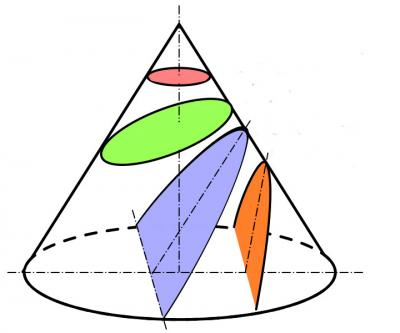
\includegraphics[width=.5\textwidth]{cone_intersection.jpg}\\
Якщо площина паралельна основі конуса, то перетин - коло;\\
Якщо площина нахилена основі конуса, то перетин - еліпс;\\
Якщо площина нахилена так, що вона паралельна твірної, то перетин - парабола;\\
Якщо площина ще сильніше нахилена, то перетин - гіпербола;
\bigline
\subsection*{Поверхні другого роду}
\defin{3.(2). Загальне рівняння поверхні другого порядку} визначається такою формулою:
\begin{align*}
a_{11}x^2 + a_{22}y^2 + a_{33}z^2 + 2a_{12}xy + 2a_{13}xz + 2a_{23}yz + b_1x + b_2y + b_3z + c = 0
\end{align*}
\lm{1.} Задана точка $M_0 = (x_0,y_0)$\\
При обертанні цієї точки навколо вісі $OX$ отримуємо коло, яке задається рівнянням:\\
$\begin{cases}
x = x_0 \\
y^2 + z^2 = y_0^2
\end{cases}
$\\
\textit{Думаю, тут все зрозуміло}\\
\begin{tikzpicture}
%plane
\draw[fill] (0.5,0,0.5) circle (1pt) node [anchor = north]{$M_0$};

\draw[thick, ->] (0,0,0)--(2,0,0) node[anchor = north, black] {$y$};
\draw[thick, ->] (0,0,0)--(0,2,0) node[anchor = east] {$z$};
\draw[thick, ->] (0,0,0)--(0,0,2) node[anchor = north east] {$x$};
\draw[dashed] (0,0,0.5) circle (0.5);
\draw[thick, ->] (-2,0.5,-2) arc (0:220:0.5);
\end{tikzpicture}
\bigline

\lm{2.} В площині $XOY$ задана така крива рівнянням $F(x,y)$, що є парною відносно $y$ (тобто крива симетрична відносно $OY$)\\
При обертанні цієї кривої навколо осі $OX$ отримуємо поверхню, яка задається рівнянням:\\
$F(x,\sqrt{y^2+z^2})=0$\\
\proof
Фіксуємо $M_0 = (x_0,y_0)$ - точку кривої. Зробимо обертання навколо $OX$, тоді отримаємо коло:\\
$\begin{cases}
x = x_0 \\
y^2 + z^2 = y_0^2
\end{cases}
$\\
Звідси $|y_0| = \sqrt{y^2+z^2}$\\
Для т. $x_0,y_0$ виконана рівність:\\
$F(x_0,y_0) = F(x_0, \sqrt{y^2+z^2}) = 0$\\
Але т. $M_0$ була довільною, тому $F(x,\sqrt{y^2+z^2})=0$, що й є бажаною поверхньою \qed
\bigline
\textbf{I. Еліпсоїд}\\
У нас вже є еліпс $\dfrac{x^2}{a^2} + \dfrac{y^2}{b^2} = 1$\\
Обертаємо навколо $OX$, тоді отримуємо:\\
$\dfrac{x^2}{a^2} + \dfrac{y^2+z^2}{b^2} = 1$\\
Отримаємо еліпсоїд обертання:\\
$\dfrac{x^2}{a^2} + \dfrac{y^2}{b^2} + \dfrac{z^2}{b^2} = 1$\\
Зробимо стискання/розтягнення вздовж осі $OZ$:\\
$z_{old} = \lambda z_{new}$\\
Тобто $\dfrac{z^2}{b^2} \to \dfrac{\lambda^2 z^2}{b^2} = \dfrac{z^2}{c^2}$\\
Отримаємо \textbf{канонічне рівняння еліпсоїда}:
\begin{align*}
\dfrac{x^2}{a^2} + \dfrac{y^2}{b^2} + \dfrac{z^2}{c^2} = 1
\end{align*}
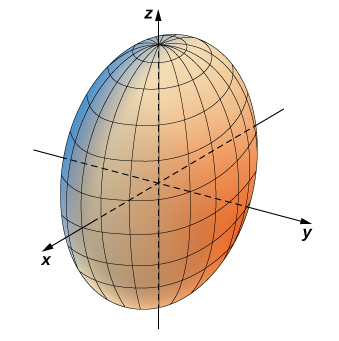
\includegraphics[scale=1]{ellipsoid.jpeg}
%
%\begin{tikzpicture}[scale = 1.5]
%\draw[->] (0,0,0) -- (2.5,0,0)node[below]{$y$};
%\draw[->] (0,0,0) -- (0,1.5,0)node[left]{$z$};
%\draw[->] (0,0,0) -- (0,0,3)node[left]{$x$};
%\draw[pattern = north east lines, pattern color = red, dashed] (-0.8,0,0) ellipse (0.3 and {sqrt(1 - 0.8*0.8/4)});
%\draw[color=red] (0,0,0) ellipse (2cm and 1cm);
%\draw[color = red, dashed](2,0,0) arc (0:180: 2cm and 0.5cm);
%\draw[color = red](-2,0,0) arc (180:360: 2cm and 0.5cm);
%\node at (2,0,0) [anchor = north west] {$b$};
%\node at (0,1,0) [anchor = south west] {$c$};
%\node at (0,0,2.3) [anchor = east] {$a$};
%\end{tikzpicture}
\bigline

\textbf{II. Гіперболоїд}\\
а) Візьмемо гіперболу $\dfrac{z^2}{c^2} - \dfrac{x^2}{a^2} = 1$\\
Обертаємо навколо $OZ$, тоді отримуємо:\\
$\dfrac{z^2}{c^2} - \dfrac{x^2+y^2}{b^2} = 1$\\
Отримаємо гіперболоїд обертання:\\
$\dfrac{z^2}{c^2} - \dfrac{x^2}{b^2} - \dfrac{y^2}{b^2} = 1$\\
Зробимо стискання/розтягнення вздовж осі $OX$:\\
$x_{old} = \lambda x_{new}$\\
Тобто $\dfrac{x^2}{b^2} \to \dfrac{\lambda^2 x^2}{b^2} = \dfrac{x^2}{a^2}$\\
Отримаємо \textbf{канонічне рівняння двопорожнинного гіперболоїда}:
\begin{align*}
\dfrac{z^2}{c^2} - \dfrac{x^2}{a^2} - \dfrac{y^2}{b^2} = 1
\end{align*}
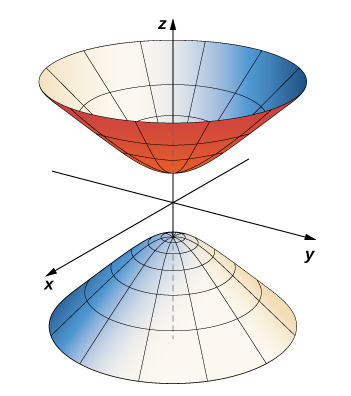
\includegraphics[scale=1]{2-shit-hyperboloid.jpeg}
\bigline

б) Візьмемо гіперболу $\dfrac{x^2}{a^2} - \dfrac{z^2}{c^2} = 1$\\
Обертаємо навколо $OZ$, тоді отримуємо:\\
$\dfrac{x^2+y^2}{a^2} - \dfrac{z^2}{c^2} = 1$\\
$\dfrac{x^2}{a^2} + \dfrac{y^2}{a^2} - \dfrac{z^2}{c^2} = 1$\\
Зробимо стискання/розтягнення вздовж осі $OY$:\\
$y_{old} = \lambda y_{new}$\\
Тобто $\dfrac{y^2}{a^2} \to \dfrac{\lambda^2 y^2}{a^2} = \dfrac{y^2}{b^2}$\\
Отримаємо \textbf{канонічне рівняння однопорожнинного гіперболоїда}:
\begin{align*}
\dfrac{x^2}{a^2} + \dfrac{y^2}{b^2} - \dfrac{z^2}{c^2} = 1
\end{align*}
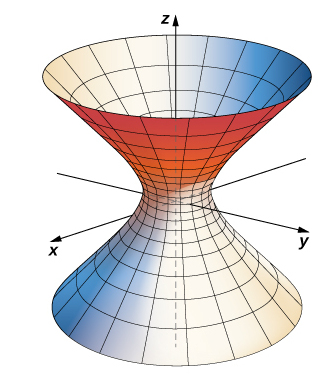
\includegraphics[scale=1]{1-shit-hyperboloid.jpeg}
\bigline
\\
\textbf{III. Параболоїд}\\
У нас вже є парабола $y^2 = 4px$\\
Обертаємо навколо $OX$, тоді отримуємо:\\
$y^2+z^2 = 4px \Rightarrow x = \dfrac{y^2}{4p} + \dfrac{z^2}{4p}$\\
Знову ті махінації з $OZ$, а також $z \to x$\\
a) Отримаємо \textbf{рівняння еліптичного параболоїду}
\begin{align*}
z = \dfrac{x^2}{a^2} + \dfrac{y^2}{b^2}
\end{align*}
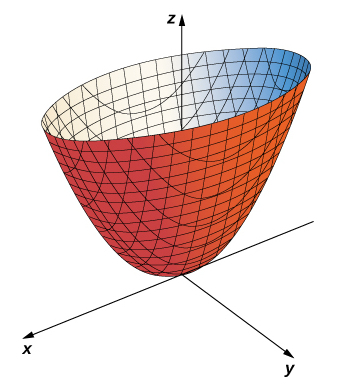
\includegraphics[scale=1]{elliptic-paraboloid.jpeg}
\\
б) Також отримаємо \textbf{рівняння гіперболічного параболоїду}
\begin{align*}
z = \dfrac{x^2}{a^2} - \dfrac{y^2}{b^2}
\end{align*}
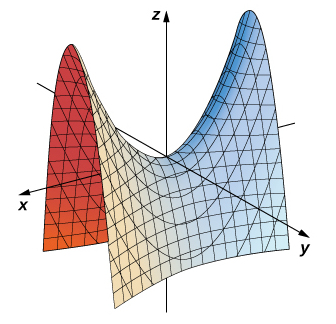
\includegraphics[scale=1]{hyperbolic-paraboloid.jpeg}
\bigline
\subsection{Циліндри}
На площині $XOY$ задана крива $F(x,y) = 0$ - основа циліндра - та пряма $l$, що перетинає основу. Через кожну точку основи $M = (x,y,0)$ проведемо пряму, паралельну $l$.\\
Отримана множина точок і є \textbf{циліндром} із основою $F(x,y) = 0$ та прямою $l$\\
\bigline
\textbf{I. Еліптичний циліндр}\\
$\vec{l} = (0,0,1)$\\
$\dfrac{x^2}{a^2} + \dfrac{y^2}{b^2} = 1$\\
Будь-яка точка, що належить еліпсу, буде належати циліндру
\bigline
\textbf{II. Гіперболічний циліндр}\\
$\vec{l} = (0,0,1)$\\
$\dfrac{x^2}{a^2} - \dfrac{y^2}{b^2} = 1$\\
Будь-яка точка, що належить гіперболі, буде належати циліндру
\bigline
\textbf{III. Параболічний циліндр}\\
$\vec{l} = (0,0,1)$\\
$y^2 = 4px$\\
Будь-яка точка, що належить параболі, буде належати циліндру
\bigline
\subsection{Конічні поверхні}
На площині $XOY$ задана крива $F(x,y) = 0$ - основа конуса - та пряма $l$, що перетинає основу. Через кожну точку основи $M = (x,y,0)$ проведемо пряму, паралельну $l$.\\
Отримана множина точок і є \textbf{циліндром} із основою $F(x,y) = 0$ та т. $K = (x_k, y_k, \underset{\neq 0}{z_k})$ - вершина конусу. Проведемо прямі, які проходять через вершину конусу $K$ та через основу\\
Отримана множина точок і є \textbf{конусом} із основою $F(x,y) = 0$ та вершиною $K = (x_k, y_k, \underset{\neq 0}{z_k})$
\bigline
\textbf{Вироджені поверхні другого роду}:\\
1) $\dfrac{x^2}{a^2} + \dfrac{y^2}{b^2} + \dfrac{z^2}{c^2} = 0$ - точка\\
2) $\dfrac{x^2}{a^2} + \dfrac{y^2}{b^2} + \dfrac{z^2}{c^2} = -1$ - уявний еліпсоїд\\
3) $(A_1 x + B_1 y + C_1 z + D_1)(A_2 x + B_2 y + C_2 z + D_2) = 0$ - пара площин
\newpage

\section{Многочлени}
\defin{5. Многочлен} - функція такого вигляду:\\
Позначення: $P_n(x) = a_n x^n + \dots + a_1x + a_0$\\
де $a_n,\dots,a_1,a_0 \in \mathbb{R}$ або $\mathbb{C}$
\bigline
Для них все зрозуміло з операціями додавання та множення многочлена на скаляр\\
\subsection{Про подільність многочленів}
\defin{5.1.1. Степеню} многочлена $f(x) = a_n x^n + \dots + a_1 x + a_0$ назвемо найвищу степінь із всіх одночленів\\
Позначення: $\deg(f(x)) = n$
\bigline
\th{5.1.2.} Для будь-яких многочленів $f(x)$ та $g(x)$ існують \underline{єдині} многочлени $s(x)$, $r(x)$, такі, що\\
$f(x) = s(x) g(x) + r(x)$\\
де $\deg(r(x)) < \deg(g(x))$ або $r(x) \equiv 0$\\
\proof
Спочатку доведемо існування:\\
I. $\deg(f(x)) < \deg(g(x))$\\
Тоді $s(x) = 0$ та $r(x) = f(x)$. Інших просто нема
\bigline
II. $\deg(f(x)) \geq \deg(g(x))$\\
Проведемо МІ за степеню $k = \deg(f(x))-\deg(g(x))$\\
$k = 0$, тобто $\deg(f(x))=\deg(g(x))=n$\\
Маємо многочлени:\\
$f(x) = a_n x^n + \dots + a_0$\\
$g(x) = b_n x^n + \dots + b_0$\\
Тоді $f(x) = \underbrace{\dfrac{a_n}{b_n}}_{=s(x)} (b_n x^n + \dots + b_0) + \\ + \underbrace{(a_{n-1}x^{n-1}+\dots+a_0 - \dfrac{a_n b_{n-1}}{b_n}x^{n-1}- \dots - \dfrac{b_0 a_n}{b_n})}_{= r(x)}$\\
Причому $\deg(r(x))=n-1<n=\deg(g(x))$
\bigline
Нехай для $k \geq 0$ існують $\tilde{s}(x), \tilde{r}(x)$
\bigline
Доведемо існування $s(x)$ та $r(x)$ для $k+1$:\\
$f(x) = a_{m+k+1} x^{m+k+1} + a_{m+k}x^{m+k} + \dots + a_0$\\
$g(x) = b_m x^m + \dots + b_0$\\
Тоді $f(x) = \dfrac{a_{m+k+1}}{b_m}x^{k+1} (b_m x^m + \dots + b_0) + \\
+ \underbrace{\left(a_{m+k}x^{m+k} + \dots + a_0 - \left(\dfrac{b_{m-1}a_{m+k+1}}{b_m}x^{m+k} + \dots + \dfrac{b_0 a_{m+k+1}}{b_m}x^k \right) \right)}_{=p(x)}$\\
Отримали $f(x) = \dfrac{a_{m+k+1}}{b_m}x^{k+1}g(x) + p(x)$\\
де $\deg(p(x)) = m+k < m+k+1 = \deg(f(x))$\\
За припущеннями МІ, для многочленів $p(x),g(x)$ існує $\tilde{s}(x), \tilde{r}(x)$, оскільки різниця степеней $= k$\\
Тоді: $p(x) = \tilde{s}(x)g(x) + \tilde{r}(x)$\\
Звідси $f(x) = \dfrac{a_{m+k+1}}{b_m}x^{k+1}g(x) + \tilde{s}(x)g(x) + \tilde{r}(x)= \\ = \underbrace{\left(\dfrac{a_{m+k+1}}{b_m}x^{k+1} + \tilde{s}(x) \right)}_{=s(x)}g(x) + \underbrace{\tilde{r}(x)}_{=r(x)}$\\
Причому $\deg(r(x)) < \deg(g(x))$ або $r(x) \equiv 0$\\
МІ доведено
\bigline
Залишилось довести єдиність\\
!Припустимо, що існують ще $s^*(x),r^*(x)$, такі, що \\ $f(x) = s^*(x)g(x) + r^*(x)$\\
Причому $\deg(r^*(x)) < \deg(g(x))$ або $r^*(x) \equiv 0$\\
Тоді $0 = f(x) - f(x) = (s(x)-s^*(x))g(x) + (r(x)-r^*(x))$\\
Або $(s(x)-s^*(x))g(x) = r^*(x)-r(x)$ \\ де $\deg(r^*(x)-r(x)) < \deg(g(x))$\\
А рівність можлива лише тоді, коли $s(x)-s^*(x) =0 \Rightarrow s(x) = s^*(x)$\\
А звідси й $r(x) = r^*(x)$. Суперечність! \qed
\bigline
\defin{5.1.3.} Число $a$ називають \textbf{коренем многочлена} $f(x)$, якщо $f(a) = 0$
\bigline
\th{5.1.4. Теорема Безу}\\
$a$ - корінь многочлена $f(x) \iff \exists h(x): f(x) = (x-a)h(x)$\\
\proof
$\boxed{\Rightarrow}$ Дано: $a$ - корінь многочлена $f(x)$, тобто $f(a) = 0$\\
Поділимо $f(x)$ на $g(x) = x-a$\\
Отримаємо: $f(x) = s(x)(x-a) + r(x)$\\
де $\deg(r(x)) < \deg(g(x)) = \deg(x-a) = 1$\\
Тоді звідси $r(x) = c$\\
Підставимо $x=a$ в наше рівняння:\\
$0 = f(a) = c$\\
Остаточно, $f(x) = \underbrace{s(x)}_{=h(x)}(x-a)$
\bigline
$\boxed{\Leftarrow}$ Дано: $\exists h(x): f(x) = (x-a)h(x)$\\
Тоді одразу $f(a) = 0 \Rightarrow$ $a$ - корень $f(x)$ \qed
\bigline
\defin{5.1.5.} Число $a$ називають \textbf{коренем многочлена} $f(x)$ \textbf{кратності} $k$, якщо $f(x) = (x-a)^k g(x)$, де $g(a) \neq 0$
\bigline
Перед теоремою зробимо деяке зауваження:\\
Розглянемо многочлен $f(x)$ степені $n$. Будь-яка функція розкладається формулою Тейлора:\\
$f(x) = f(a) + \dfrac{f'(a)}{1!}(x-a) + \dots + \dfrac{f^{(n)}(a)}{n!}(x-a)^n + \dfrac{f^{(n+1)}(\theta)}{(n+1)!}(x-a)^{n+1}$\\
Через те, що $\deg(f(x)) = n$, маємо, що $f^{(n+1)}(x) = 0$ \\ Тоді остаточно отримаємо іншу репрезентацію многочлена:\\
$f(x) = f(a) + \dfrac{f'(a)}{1!}(x-a) + \dots + \dfrac{f^{(n)}(a)}{n!}(x-a)^n$
\bigline
\th{5.1.6. Критерій кратності кореня}\\
$a$ - корінь кратності $k$ многочлена $f(x) \iff f(a)=f'(a)=\dots=f^{(k-1)}(a) =0$, але $f^{(k)}(a) \neq 0$\\
\proof
$\boxed{\Rightarrow}$ Дано: $a$ - корінь кратності $k$ для $f(x)$, тобто:\\
$f(x) = (x-a)^k g(x)$, де $g(a) \neq 0$\\
Більш того, якщо $\deg(f(x)) = n$, то звідси $\deg(g(x)) = n-k$\\
Тому розкладемо функцію $g(x)$ за щойно отриманою формулою:\\
$f(x) = (x-a)^k \left(g(a) + \dfrac{g'(a)}{1!}(x-a) + \dots + \dfrac{g^{(n-k)}(a)}{(n-k)!}(x-a)^{n-k} \right) = \\
= (x-a)^k g(a) + (x-a)^{k+1}\dfrac{g'(a)}{1!} + \dots + (x-a)^n\dfrac{g^{(n+k)}(a)}{(n+k)!}$\\
Але з іншого боку:\\
$f(x) = f(a) + \dfrac{f'(a)}{1!}(x-a) + \dots + \dfrac{f^{(k-1)}(a)}{(k-1)!}(x-a)^{k-1} + \dfrac{f^{(k)}(a)}{k!}(x-a)^{k} + \dots + \dfrac{f^{(n)}(a)}{n!}(x-a)^n$\\
В першому рівності многочлен починався зі степені $k$, тому й друга рівність має починатись зі степені $k$, звідси й\\
$f(a) = 0 \hspace{0.5 cm} \dfrac{f'(a)}{1!} = 0 \hspace{0.5 cm} \dots \hspace{0.5 cm} \dfrac{f^{(k-1)}(a)}{k!} = 0$\\
При цьому $\dfrac{f^{(k)}(a)}{k!} \neq 0$. Отже, отримали бажану умову
\bigline
$\boxed{\Leftarrow}$ Дано: $f(a)=f'(a)=\dots=f^{(k-1)}(a) =0$, але $f^{(k)}(a) \neq 0$\\
Розкладемо нашу функцію $f$ за формулою:\\
$f(x) = f(a) + \dfrac{f'(a)}{1!}(x-a) + \dots \dfrac{f^{(k-1)}(a)}{(k-1)!}(x-a)^{k-1} + \dfrac{f^{(k)}(a)}{k!}(x-a)^{k} + \dots + \dfrac{f^{(n)}(a)}{n!}(x-a)^n$\\
Тоді\\
$f(x) = \dfrac{f^{(k)}(a)}{k!}(x-a)^{k} + \dots + \dfrac{f^{(n)}(a)}{n!}(x-a)^n = \\ = (x-a)^k \underbrace{\left(\dfrac{f^{(k)}(a)}{k!} + \dots + \dfrac{f^{(n)}(a)}{n!}(x-a)^{n-k} \right)}_{=g(x)}$\\
Через те, що $f^{(k)}(a) \neq 0$, то звідси $g(a) \neq 0$, отже:\\
$f(x) = (x-a)^k g(x) \Rightarrow$ $a$ - корінь кратності $k$ \qed
\bigline
\subsection{Комплексні корені многочленів}
\prp{5.2.1.} Якщо $z \in \mathbb{C}$ є коренем многочлена $f(x)$ з дійсними коефіцієнтами, то $\bar{z}$ - теж корінь\\
\proof
Задано многочлен:
$f(x) = a_n x^n + \dots + a_0$\\
де $f(z) = 0$\\
Тоді маємо:\\
$f(\bar{z}) = a_n \bar{z}^n + \dots + a_0 = \overline{a_n z^n} + \dots + \overline{a_0} = \overline{a_n z^n + \dots + a_0} = \overline{f(z)} = \bar{0} = 0$ \qed
\bigline
\prp{5.2.2.} Корені $z$ та $\bar{z}$ мають однакову кратність\\
\proof
Нехай $z$ - корінь кратності $k$, тобто $f(z) = f'(z) = \dots = f^{(k-1)}(z) = 0, f'^{(k)}(z) \neq 0$\\
Тоді за міркуваннями минулого твердження,\\
$f(\bar{z}) = f'(\bar{z}) = \dots = f^{(k-1)}(\bar{z}) = 0, f'^{(k)}(\bar{z}) \neq 0$ \\ Отже, $\bar{z}$ - корінь кратності $k$ \qed
\bigline
\th{5.2.3. Основна теорема алгебри}\\
У многочлена з комплексними коефіцієнтами є принаймні один корень $z_0 \in \mathbb{C}$\\
\textit{Без доведення}
\bigline
\crl{5.2.3.} Заданий многочлен степені $n$ з комплексними коефіцієнтами. Тоді має $n$ коренів, враховуючи кратність\\
\proof
Нехай $z_1$ - корінь $f(z) \Rightarrow f(z) = (z-z_0)^{k_1} g(z)$, причому $g(z_1) \neq 0$\\
За основною теоремою алгебри, $g(z)$ має корінь $z_2 \Rightarrow \\ g(z) = (z-z_0)^{k_2} g_2(z)$, причому $g_2(z_2) \neq 0$\\
І знову за основною теоремою алгебри, $g_2(z)$ має корінь $z_3 \dots$\\
Тому остаточно отримуємо:\\
$f(z) = A_0(z-z_1)^{k_1}(z-z_2)^{k_2}\dots(z-z_m)^{k_m}$, де\\
$k_1 + k_2 + \dots + k_m = n = \deg(f(z))$ \qed
\bigline
\th{5.2.4.} Функція $f(x)$ з дійсними коефіцієнтами розкладається на прості множники:\\
$f(x) = A_0 (x-a_1)^{k_1} \dots (x-a_m)^{k_m} (x^2+p_1x+q_1)^{s_1} \dots (x^2+p_j+q_j)^{s_j}$\\
де $k_1 + \dots + k_m + 2s_1 + \dots + 2s_j = n = \deg(f(x))$\\
Більш того, всі дискримінанти квадратних рівнянь - від'ємні \\
$a_1, \dots a_m \in \mathbb{R}$\\
\proof
За попереднім наслідком,\\
$f(x) = A_0(x-a_1)^{k_1} \dots (x-a_m)^{k_m} (x-z_1)^{s_1} (x-\bar{z_1})^{s_1} \dots (x-z_j)^{s_j} (x-\bar{z_j})^{s_j}$\\
Розпишемо такі добутки:\\
$(x-z_1)(x-\bar{z_1}) = x^2 - x(z_1 +\bar{z_1}) + z_1 \bar{z_1} =$\\
$z_1 + \bar{z_1} = 2 \Re z_1 \overset{\textrm{позн.}}{=} -p_1 \in \mathbb{R}$\\
$z_1 \bar{z_1} = (\Re z_1)^2 + (\Im z_1)^2 \overset{\textrm{позн.}}{=} q_1 \in \mathbb{R}$\\
$= x^2 + p_1x + q_1$, для якого $D < 0$ (тому що фактично 2 корені є комплексними)\\
І так з рештою. Тому\\
$f(x) = A_0 (x-a_1)^{k_1} \dots (x-a_m)^{k_m} (x^2+p_1x+q_1)^{s_1} \dots (x^2+p_j+q_j)^{s_j}$ \qed
\bigline
\subsection{Спільні дільники та кратні двох многочленів}
\defin{5.3.1.(1)} Многочлен $h(x)$ називається \textbf{дільником} $f(x)$, якщо $f(x) = s(x)h(x) + 0$
\bigline
\defin{5.3.1.(2)} Многочлен $h(x)$ називається \textbf{спільним дільником} $f(x)$ та $g(x)$, якщо він є дільником кожного
\bigline
\defin{5.3.1.(3)} Многочлен $d(x)$ називається \textbf{\underline{найбільшим} спільним дільником} $f(x)$ та $g(x)$, якщо він ділиться без остачі на будь-який спільний дільник $f(x)$ та $g(x)$\\
Позначення: $d(x) = \textrm{GCD}(f,g)$
\bigline
\prp{5.3.2.} Нехай $d_1$ та $d_2$ - НСД $f(x)$ та $g(x)$\\
Тоді $\exists c \in \mathbb{R}: d_1(x) = cd_2(x)$\\
\proof
Якщо $d_1(x) = \textrm{GCD}(f,g)$ та $d_2$ - спільний дільник $f,g$, то $d_1$ ділиться націло на $d_2$, тобто\\ $d_1(x) = s_1(x) d_2(x)$ $(*)$\\
Якщо $d_2(x) = \textrm{GCD}(f,g)$ та $d_1$ - спільний дільник $f,g$, то $d_2$ ділиться націло на $d_1$, тобто\\$d_2(x) = s_2(x) d_1(x)$ $(**)$\\
Повернемось до рівняння $(*)$:\\
$\Rightarrow d_1(x) = s_1(x) d_2(x) \overset{(**)}{=} s_1(x)s_2(x)d_1(x)$\\
$\Rightarrow s_1(x)s_2(x) = 1 \Rightarrow s_1(x) = c_1, s_2(x) = c_2$\\
Отже, $d_1(x) = c_1 d_2(x)$ \qed
\bigline
\rm{5.3.2.} $d(x) = \textrm{GCD}(f,g) \Rightarrow \forall c \in \mathbb{R}: c d(x) = \textrm{GCD}(f,g)$\\
Дійсно, $f(x) = s_1(x)d(x) \Rightarrow f(x) = \dfrac{s_1(x)}{c} cd(x)$\\
Також $g(x) = s_2(x)d(x) \Rightarrow g(x) = \dfrac{s_2(x)}{c} cd(x)$
\bigline
\textbf{Алгоритм Евкліда, для пошуку НСД}\\
Задані $f(x)$ та $g(x)$\\
1) $f(x) = s_1(x) g(x) + r_1(x)$\\
2) $g(x) = s_2(x) r_1(x) + r_2(x)$\\
3) $r_1(x) = s_3(x) r_2(x) + r_3(x)$\\
\dots \\
n) $r_{n-2}(x) = s_n(x)r_{n-1}(x) + r_n(x)$\\
Зауважимо, що $\textrm{deg}(r_1(x)) > \textrm{deg}(r_2(x)) > \dots > \textrm{deg}(r_n(x))$\\
Тобто наш алгоритм точно є скінченним\\
n+1) $r_{n-1}(x) = s_{n+1}(x)r_n(x) + 0$\\
Таким чином, ми отримаємо:\\
$r_n(x) = \textrm{GCD}(f,g)$\\
Маємо наступне твердження:\\
\prp{5.3.3.} $\textrm{GCD}(f,g) = r_n(x)$\\
\proof
Покажемо, що $r_n(x)$ - спільний дільник $f,g$\\
Дійсно, якщо $r_{n-1}$ підставити в 'n)', потім $r_{n-2}$ - в 'n-1)' і так до кінця, то отримаємо, що $f \vdots r_{n}$\\
Покажемо, що $r_n(x)$ - НСД $f,g$\\
Дійсно, якщо $d$ - довільний спільний дільник $f,g$, то звідси $r_1 \vdots d$, $r_2 \vdots d$, \dots, $r_n \vdots d$\\
Таким чином, $r_n(x) = \textrm{GCD}(f,g)$ \qed
\bigline
\prp{5.3.4.} Нехай $d(x)$ - довільний дільник $f(x),g(x)$\\
Тоді $\deg(d(x)) > \deg(\textrm{GCD}(f,g))$
\bigline
\defin{5.3.5.(1)} Многочлен $m(x)$ називається \textbf{спільним кратним} $f(x)$ та $g(x)$, якщо $m(x)$ ділиться на $f(x)$ та $g(x)$ одночасно
\bigline
\defin{5.3.5.(2)} Многочлен $M(x)$ називається \textbf{\underline{найменшим} спільним кратним} $f(x)$ та $g(x)$, якщо він ділиться без остачі на будь-яке спільне кратне $f(x)$ та $g(x)$\\
Позначення: $M(x) = \textrm{LCM}(f,g)$
\bigline
\textbf{Знаходження НСК}\\
I. Знайти $\textrm{GCD}(f,g) = d(x)$, тобто\\
$f(x) = f_1(x) d(x)$\\
$g(x) = f_2(x) d(x)$\\
II. Тоді $k(x) = f_1(x)f_2(x)d_2(x)$\\
Це є спільним кратним $f(x)$ та $g(x)$\\
Будь-яке спільне кратне повинно ділитись на $f(x)$ та $g(x)$, а отже, й на $f_1(x)f_2(x)d(x) = k(x)$\\
Звідси отримуємо\\
$\textrm{LCM}(f,g) = \dfrac{f(x)g(x)}{\textrm{GCD}(f,g)}$
\bigline
\prp{5.3.6.} Нехай $k_1$ та $k_2$ - НСК $f(x)$ та $g(x)$\\
Тоді $\exists c \in \mathbb{R}: k_1(x) = ck_2(x)$\\
\proof
Скористаємось отриманою щойно формулою\\
Коли $k_1(x) = \textrm{LCM}(f,g)$, то $d_1(x) = \textrm{GCD}(f,g) = \dfrac{f(x)g(x)}{k_1(x)}$\\
Коли $k_2(x) = \textrm{LCM}(f,g)$, то $d_2(x) = \textrm{GCD}(f,g) = \dfrac{f(x)g(x)}{k_2(x)}$\\
Але оскільки $d_1(x) = c^*d_2(x)$, то звідси $\dfrac{1}{k_1(x)} = \dfrac{c^*}{k_2(x)} \Rightarrow k_1(x) = c k_2(x)$ \qed
\bigline
\subsection{Дробово-раціональні вирази, розклад}
\defin{5.4.1.(1)} \textbf{Дробово-раціональним виразом} називають $\dfrac{P(x)}{Q(x)}$, де $P(x),Q(x)$ - многочлени
\bigline
\defin{5.4.1.(2)} \textbf{Простими дробами} називають один із дробово-\\раціональних виразів
\begin{align*}
\dfrac{1}{x-a} \hspace{1cm} \dfrac{1}{(x-a)^k} \hspace{1cm} \dfrac{Ax+B}{x^2+px+q} \hspace{1cm} \dfrac{Ax+B}{(x^2+px+q)^k}
\end{align*}
Останні два дроби - це в дійсному випадку. Ба більше, дискриминанти знаменників - від'ємний
\bigline
\textbf{Розклад дробово-раціональних виразів на суму простих дробов}\\
1) Якщо $\deg(P(x)) \geq \deg(Q(x))$, то ділимо одне одного, тобто\\
$P(x) = S(x)Q(x) + P_1(x)$\\
Звідси $\dfrac{P(x)}{Q(x)} = S(x) + \dfrac{P_1(x)}{Q(x)}$\\
Тут $\deg(P_1(x)) < \deg(Q(x))$
\bigline
2) Якщо $\deg(P(x)) < \deg(Q(x))$\\
Вже відомо, що \\ $Q(x) = E(x-a_1)^{k_1} \dots (x-a_m)^{k_m} (x^2+p_1x+q_1)^{l_1} \dots (x^2+p_s x+q_s)^{l_s}$ - розклад
\bigline
\lm{5.4.2.(1)} Нехай $\dfrac{P(x)}{Q(x)}$, $\deg(P(x)) < \deg(Q(x))$\\
$Q(x) = (x-a)^k Q_1(x)$, де $Q_1(a) \neq 0$\\
Тоді $\exists A \in \mathbb{R}: \exists P_1(x): \deg(P_1(x)) < \deg(P(x))$ та $P_1(a) \neq a:$\\
$\dfrac{P(x)}{Q(x)} = \dfrac{A}{(x-a)^k} + \dfrac{P_1(x)}{(x-a)^{k-1}Q_1(x)}$\\
\proof
Хочемо знайти $A$ та $P_1(x)$, таку, що\\
$\dfrac{P(x)}{(x-a)^kQ_1(x)} = \dfrac{A}{(x-a)^k} + \dfrac{P_1(x)}{(x-a)^{k-1}Q_1(x)}$\\
$\dfrac{P(x)}{(x-a)^k Q_1(x)} = \dfrac{AQ_1(x)+P_1(x)(x-a)}{(x-a)^kQ_1(x)}$\\
$P(x) = AQ_1(x) + P_1(x)(x-a)$ - виконується $\forall x$\\
Тому для $x=a$ випливає, що $P(a) = AQ_1(x) \Rightarrow A = \dfrac{P(a)}{Q_1(a)}$\\
Крім того, $P_1(x)(x-a) = P(x) - AQ_1(x)$\\
Оскільки $P(a) - AQ_1(a) = 0$, то $P(x) -AQ_1(x) = P_1(x)(x-a)$\\
Тобто $P_1(x)$ отримується діленням $P(x)-AQ_1(x)$ на $(x-a)$ \qed
\bigline
\lm{5.4.2.(2)} Задано $\dfrac{P(x)}{Q(x)}$, $\deg(P(x)) < \deg(Q(x))$\\
$Q(x) = (x^2+px+q)^kQ_1(x)$\\
Тоді $\exists A,B \in \mathbb{R}: \exists P_1(x): \deg(P_1(x)) < \deg(P(x))$ та $P(x)$ не ділиться на $x^2+px+q:$\\
$\dfrac{P(x)}{Q(x)} = \dfrac{Ax+B}{(x^2+px+q)^k} + \dfrac{P_1(x)}{(x^2+px+q)^{k-1}Q_1(x)}$\\
\proof
Хочемо знайти $A,B$ та $P_1(x)$, таку, що\\
$\dfrac{P(x)}{(x^2+px+q)^k Q_1(x)} = \dfrac{Ax+B}{(x^2+px+q)^k} + \dfrac{P_1(x)}{(x^2+px+q)^{k-1}Q_1(x)}$\\
$\dfrac{P(x)}{(x^2+px+q)^k Q_1(x)} = \dfrac{P(x)}{(x^2+px+q)^k Q_1(x)} = \dfrac{(Ax+B)Q_1(x)+P_1(x)(x^2+px+q)}{(x^2+px+q)^k Q_1(x)}$\\
$P(x) = (Ax+B)Q_1(x)+P_1(x)(x^2+px+q)$ $(*)$\\
Нехай $z_0$ та $\bar{z_0}$ - корені $x^2+px+q$\\
Оскільки $P(x)$ Та $Q(x)$ не діляться на $x^2+px+q$, то \\ $P(z_0) \neq 0, Q(z_0) \neq 0,P(\bar{z_0}) \neq 0, Q(\bar{z_0}) \neq 0$\\
Підставимо $z_0, \bar{z_0}$ в $(*)$\\
$\begin{cases}
P(z_0) = (Az_0+B)Q_1(z_0) \\
P(\bar{z_0}) = \overline{P(z_0)} = (A\bar{z_0}+B)Q_1(\bar{z_0}) = (A\bar{z_0}+B)\overline{Q_1(z_0)}
\end{cases}
$\\
Додамо два рівняння, також віднімемо та поділемо на $i$, тоді:\\
$\begin{cases}
2 \Re P(z_0) = 2A \Re (z_0 Q_1(z_0)) + 2B \Re Q(z_0) \\
2 \Im P(z_0) = 2 \Im(z_0 Q_1(z_0)) + 2B \Im Q(z_0)
\end{cases}
$\\
Ну а далі шукаємо $A,B$, які будуть дійсними\\
Повернемось до рівняння:\\
$P(x) = (Ax+B)Q_1(x) + P_1(x)(x^2+px+q)$\\
$A,B$ вже маємо\\
$P_1(x)(x^2+px+q) = P(x) - (Ax+B)Q_1(x) $\\
Корені $z_0, \bar{z_0}$ многочлена $x^2+px+q$ є коренями $P(x)-(Ax+B)Q_1(x)$\\
Тому $P(x) - (Ax+B)Q_1(x)$ ділиться на $x^2+px+q$\\
Остаточно знайдемо $P_1(x)$ \qed
\bigline
\th{5.4.3.} Задано $\dfrac{P(x)}{Q(x)}$, $\deg(P(x)) < \deg(Q(x))$ \\ $Q(x) = E(x-a_1)^{k_1} \dots (x-a_m)^{k_m} (x^2+p_1x+q_1)^{l_1} \dots (x^2+p_s x+q_s)^{l_s}$\\
Тоді
$\dfrac{P(x)}{Q(x)} = \dfrac{A_{11}}{(x-a_1)} + \dots + \dfrac{A_{1k_1}}{(x-a_1)^{k_1}} + \dfrac{A_{21}}{(x-a_2)} + \dots + \dfrac{A_{2k_2}}{(x-a_2)^{k_2}} + \dots \\ + \dfrac{A_{m1}}{(x-a_m)} + \dots + \dfrac{A_{mk_m}}{(x-a_m)^{k_m}} + \dfrac{B_{11}x + C_{11}}{x^2+p_1x+q_1} + \dots + \dfrac{B_{1l_1}x + C_{1l_1}}{(x^2+p_1x+q_1)^{l_1}} + \dots + \dfrac{B_{s1}x + C_{s1}}{x^2+p_s x+q_s} + \dots + \dfrac{B_{sl_s}x + C_{sl_s}}{(x^2+p_s x+q_s)^{l_s}}$\\
\textit{Ґрунтується на попередньо доведених лем}\\
$\scaleobj{5}{\blacksquare}$\\
\end{document}
